% !TEX root = ../main.tex

%************************************************
\chapter{Quasar-driven outflows in the narrow line region}
\label{ch:nlr} 
%************************************************

\section{Introduction}

X-ray and ultra-violet spectroscopy has revealed high-velocity outflows to be nearly ubiquitous in high accretion rate quasars.
Strong evidence for high-velocity outflows include BALs, NALs and blueshifts in high-ionisation broad emission-lines. 
This suggests that the energy released by quasars can have a dramatic effect on their immediate environment. 

The BH mass and the mass of the host-galaxy spheroid are strongly correlated.
This suggests that the BH and bulge grown synchronously, with the energetic output of the rapidly-accreting BH coupling with the gas in the host-galaxy and regulating star formation and the growth of the BH itself \citep[e.g.][]{silk98,king03,dimatteo05,king15}.
If this picture is true, then quasars should be capable of driving powerful outflows over galactic scales. 
In recent years, a huge amount of resources have been devoted to searching for observational evidence of these galaxy-wide, quasar-driven outflows. 
This has resulted in recent detections of outflows in quasar-host galaxies using tracers of atomic, molecular, and ionised gas \citep[e.g.][]{nesvadba06,arav08,nesvadba08,moe09,dunn10,alexander10,harrison12,harrison14,nesvadba10,rupke13,veilleux13,nardini15,feruglio10,alatalo11,cimatti13,cicone14}.  

One particularly successful technique has been using forbidden emission-lines to probe conditions in the AGN NLR. 
Because of its high equivalent width, [\ion{O}{III}]\ll$4960,5008$ is the most studied of the narrow AGN emission-lines. 
The [\ion{O}{III}] emission is found to consist of two distinct components: a narrow, `core' component, with a velocity close to the systemic redshift of the host-galaxy, and a broader `wing' component, which is normally blueshifted. 
The general consensus is that the core component is dominated by the gravitational potential of the host-galaxy whereas the broad, blueshifted wing traces outflowing gas. 
The relative balance between the core and wing components varies significantly from object to object, and may depend on properties of the AGN \citep[e.g. luminosity;][]{shen14}. 

Observations of broad velocity-widths and blueshifts in narrow emission-lines stretch back several decades \citep[e.g.][]{weedman70,stockton76,heckman81,veron81,feldman82,heckman84,vrtilek85,whittle85,boroson92}. 
However, these studies rely on small samples, which are often unrepresentative of the properties of the AGN population. 
More recently, the advent of large optical spectroscopic surveys (e.g. SDSS) have facilitated studies of the NLR in tens of thousands of AGN \citep[e.g.][]{boroson05,greene05a,zhang11,mullaney13,zakamska14,shen14}. 
This has provided constraints on the prevalence and drivers of ionised outflows.   
At the same time, there is strong evidence from spatially resolved spectroscopic observations that these outflows are extended over galaxy scales \citep[e.g.][]{greene09,greene11,hainline13,harrison12,harrison14}. 

However, these studies do not cover the redshift range when star formation and BH accretion peaked ($2 \lesssim z \lesssim 4$), which is when quasar feedback is predicted to be at its most effective.  
At these redshifts bright optical emission-lines including the [\ion{O}{III}] doublet are redshifted to near-infrared wavelengths, where observations are much more challenging. 
As a consequence, studies at high redshifts have typically relied on relatively small numbers of objects \citep[e.g.][]{netzer04,sulentic04,shen16a}.
These studies find [\ion{O}{III}] to be broader in more luminous AGN, suggesting that AGN efficiency in driving galaxy-wide outflows increases with luminosity \citep[e.g.][]{netzer04,nesvadba08,kim13,brusa15,carniani15,perna15,bischetti16}. 
The fraction of objects with very weak [\ion{O}{III}] emission also appears to increase with redshift and/or luminosity \citep[e.g.][]{netzer04}. 

Other recent studies have looked at the [\ion{O}{III}] emission properties of extreme objects - e.g. heavily obscured quasars \citep{zakamska16} and the most luminous quasars \citep{bischetti16} - at redshifts $z\sim2$. 
When detected, the [\ion{O}{III}] emission in these objects is extremely broad and strongly blueshifted. 
These observations are consistent with galaxy formation models that predict AGN feedback to be strongest in luminous, dust-obscured quasars.

In this chapter we analyse the [\ion{O}{III}] properties of a sample of $354$ high-luminosity, redshift $1.5 < z < 4$ quasars.
To date, this is the largest study of the NLR properties of high redshift quasars. 

\section{Quasar sample}

From our near-infrared spectroscopic catalogue (Chapter~\ref{ch:nirsample}), we have selected $354$ quasars which have spectra covering the strong, narrow [\ion{O}{III}] doublet. 
The broad Balmer \hb line has also been observed for all but two of the sample. 
For $165$ quasars, the spectra extend to the broad \ha emission-line at $6565$\,\AA, and in $260$ objects optical spectra, including \ion{C}{IV}, are also available (mostly from SDSS/BOSS). 
The sample covers a wide range in redshifts ($1.5 \lesssim z \lesssim 4$) and luminosities ($45.5 \lesssim \log L_{\mathrm Bol} \lesssim 49$\,\ergs). 
The spectrographs and telescopes used to obtain the near-infrared spectra are summarised in Table~\ref{tab:specnums_ch4}.

\begin{table}
  \centering
  \footnotesize 
  \caption{The numbers of quasars with [\ion{O}{III}] line measurements and the spectrographs and telescopes used to obtain the near-infrared spectra.}
  \label{tab:specnums_ch4}
    \begin{tabular}{ccc} 
    \hline
    Spectrograph & Telescope & Number \\
                 &           & \\
    \hline
    FIRE         & MAGELLAN  & $31$ \\
    GNIRS        & GEMINI-N  & $28$ \\
    ISAAC        & VLT       & $7$ \\
    LIRIS        & WHT       & $7$ \\
    NIRI         & GEMINI-N  & $29$ \\
    NIRSPEC      & Keck II   & $3$ \\
    SINFONI      & VLT       & $80$ \\
    SOFI         & NTT       & $76$ \\
    TRIPLESPEC   & ARC-$3.5$m  & $27$ \\
    TRIPLESPEC   & P$200$      & $45$ \\
    XSHOOTER     & VLT       & $21$ \\
    \hline
    \multicolumn{2}{c}{Total} & $354$ \\
    \hline
    \end{tabular}
\end{table} 

\section{Parametric model fits}

In this section, we describe how emission-line parameters are derived. 
Our approach is to model the spectra using a power-law continuum, an empirical \ion{Fe}{II} template (taken from \citealt{boroson92}) and multiple Gaussian components to model the emission from the broad and narrow emission-line regions.
Non-parametric properties are then derived from the best-fitting model. 
This approach, which is commonly adopted in the literature \citep[e.g.][]{shen11,shen12,shen16a}, is more robust when analysing spectra with limited S/N (in comparison to measuring line properties directly from the data) and allows different emission-lines to be de-blended.

The same approach was used to model the \hbns/[\ion{O}{III}] complex in Chapter~\ref{ch:bhmass}. 
However, a number of small adjustments have been made to the model (Section~\ref{sec:oiiimodel}). 
\ha emission-line properties (used to estimate the quasar systemic redshift) are also re-derived in this chapter using a slightly modified model (Section~\ref{sec:hamodel}) to the one adopted in Chapter~\ref{ch:bhmass}. 
\ion{C}{IV} emission-line properties (used to infer the strength of BLR outflows) are taken directly from Chapter~\ref{ch:bhmass}. 

\subsection{Transforming spectra to the quasar rest-frame}

Before a spectrum can be modelled, it must first be transformed to the quasar rest-frame.  
The redshift used in this transformation is either derived from the peak of the broad \ha emission ($\sim40$ per cent of our sample), from the peak of the broad \hb emission ($\sim40$ per cent) or from the peak of the narrow [\ion{O}{III}] emission ($20$ per cent).
The rest-frame transformation is only required to be accurate to within $\sim1000$\,\kms\, of the systemic redshift for our fitting procedure to work. 
In later sections, more precise estimates of the systemic redshift will be calculated using our parametric model fits. 

\subsection{Removing \ion{Fe}{II} emission}

\begin{figure}
    \centering
    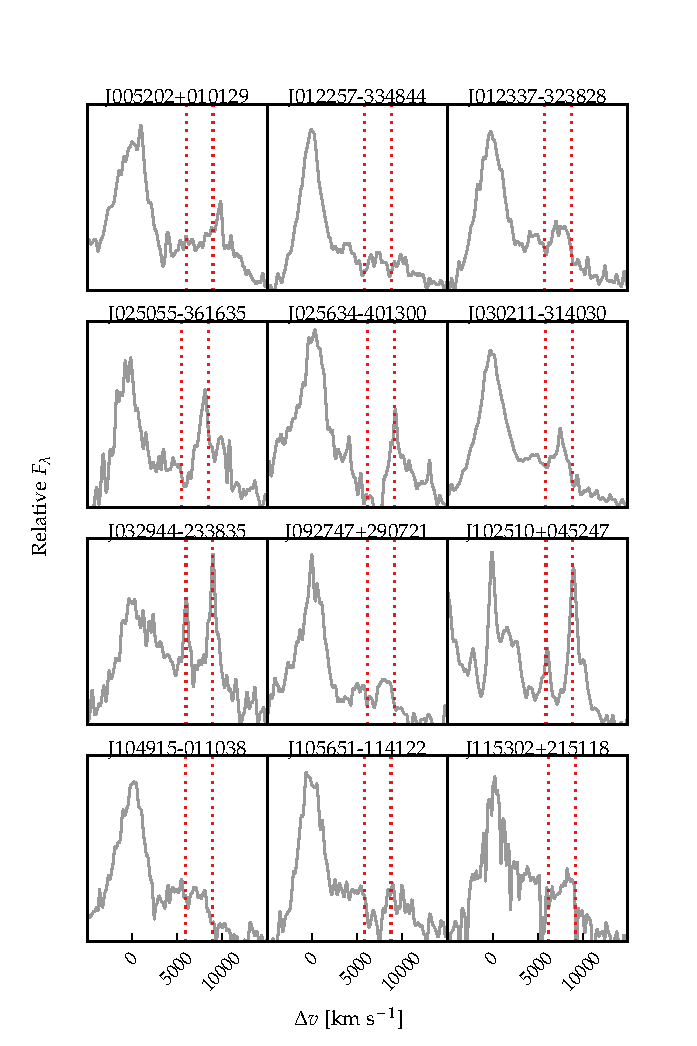
\includegraphics[width=\columnwidth]{figures/chapter04/example_spectrum_grid_extreme_fe_1.pdf} 
    \caption[{Spectra of the $24$ objects for which significant \ion{Fe}{II} emission is still visible following our \ion{Fe}{II}-subtraction procedure.}]{Spectra of the $24$ objects for which significant \ion{Fe}{II} emission is still visible following our \ion{Fe}{II}-subtraction procedure. Spectra have been smoothed via convolution with a $100$\,\kms\, Gaussian kernel. The vertical lines indicate the expected positions of the [\ion{O}{III}] doublet (which is generally very weak) with the systemic redshift defined using the peak of the broad \hb emission.}     
    \label{fig:bad_fe}
\end{figure}

\begin{figure}
\ContinuedFloat
    \centering
    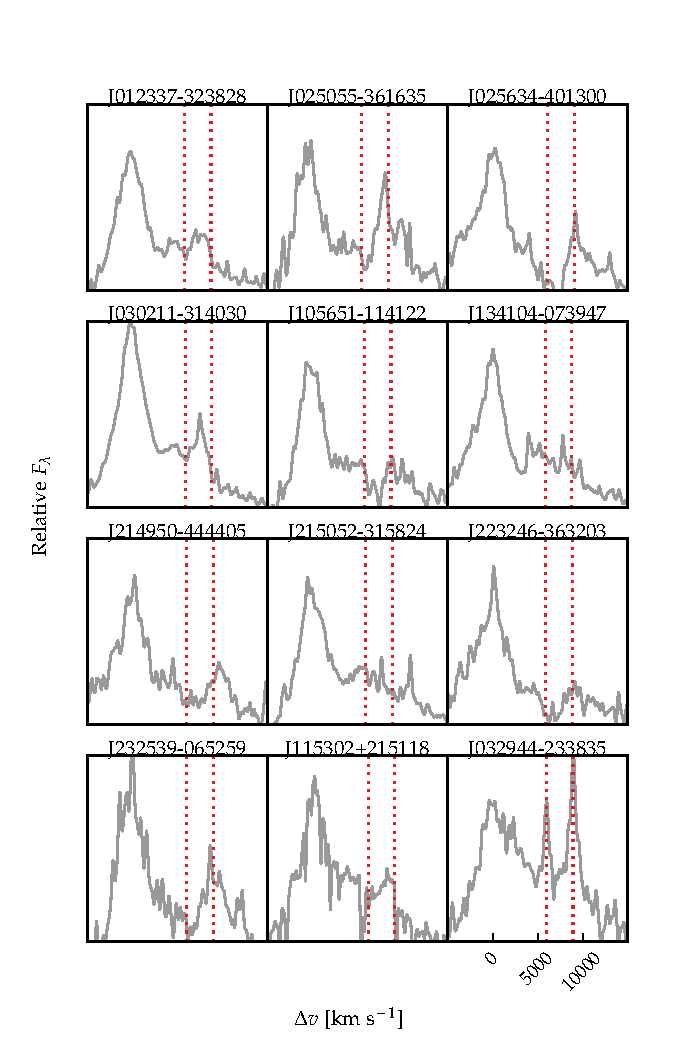
\includegraphics[width=\columnwidth]{figures/chapter04/example_spectrum_grid_extreme_fe_2.pdf} 
    \caption[]{Continued.}     
\end{figure}


\ion{Fe}{II} emission is generally strong in the vicinity of \hbns/[\ion{O}{III}]. 
Therefore, before \hbns/[\ion{O}{III}] is modelled, we first model and subtract the continuum and \ion{Fe}{II} emission using the procedure described in Chapter~\ref{ch:bhmass}. 

We encountered $24$ objects for which \ion{Fe}{II} emission appears to be present in the spectrum even after the subtraction procedure (Figure~\ref{fig:bad_fe}).  
In these objects the relative strengths of the \ion{Fe}{II} lines differ significantly from those of I Zw $1$, on which the \citet{boroson92} \ion{Fe}{II} template we use is based. 
The residual \ion{Fe}{II} emission is at rest-frame wavelengths very close to zero-velocity wavelengths of the [\ion{O}{III}] doublet, which is generally very weak in these objects. 
The Gaussians we fit to the spectra to model [\ion{O}{III}] are therefore strongly biased, and the [\ion{O}{III}] emission properties we infer from the model are in error by large factors. 

For example, J$223819$-$092106$ was analysed by \citet{shen16a} using a very similar model. 
\citet{shen16a} reported the [\ion{O}{III}] emission in this object to be shifted by $\sim7500$\,\kms\, relative to the \citet{hewett10} systemic redshift. 
Our analysis suggests that emission which was modelled by \citet{shen16a} as [\ion{O}{III}] is more likely to be poorly-subtracted \ion{Fe}{II} emission.  
Because the derived [\ion{O}{III}] emission properties can be strongly biased in objects so-affected, these objects are flagged and are excluded from our analysis in the remainder of this chapter (leaving $330$ objects in our sample). 

\subsection{Modelling \hbns/[\ion{O}{III}]}
\label{sec:oiiimodel}

The \hb and [\ion{O}{III}] emission is fit using a similar procedure to the one described in Chapter~\ref{ch:bhmass}. 
However, we make a number of modifications to the parametric model employed, which we will now describe. 

\subsubsection{\hb}

\begin{table}
  \centering
  \footnotesize 
  \caption{Summary of models used to fit the \hb emission, and the number of quasars each model is applied to.}
  \label{tab:hbmod}
    \begin{tabular}{ccc} 
    \hline
    Model & Fix centroids? & Number \\
    \hline
    $2$ broad Gaussians + $1$ narrow Gaussian & No & $9$ \\
    $2$ broad Gaussians & No  &  $274$ \\
    $2$ broad Gaussians & Yes &  $39$ \\
    $1$ broad Gaussian  & N/A &  $8$ \\
    \hline
    \end{tabular}
\end{table} 

In general, \hb is modelled by two Gaussians with non-negative amplitudes and FWHM greater than $1200$\,\kms.
In $10$ objects \hb is modelled with a single Gaussian and in $41$ objects \hb is modelled with two Gaussians, but the velocity centroids of the two Gaussians are constrained to be equal. 
These spectra generally have low S/N, and adding extra freedom to the model does not significantly decrease the  reduced $\chi^2$.
In addition there are cases where the blue wing of the \hb emission is below the lower wavelength limit of the spectra; in these cases models with more freedom are insufficiently constrained by the data.    

Contributions to the \hb emission from the NLR is weak in the vast majority of our sample, and in general we do not include an additional Gaussian component to model this emission. 
In nine objects features in the model - data residuals suggest that a narrow emission component is significant, and an additional narrow Gaussian is included for these quasars. 
It is likely that there is some not insignificant contribution from the NLR in other quasars in our sample. 
If this is the case then measures of the \hb velocity width will be biased to lower values on average. 
However, our systemic redshift estimates that use the peak of the \hb emission (Section~\ref{sec:ch4_redshifts}) will not be affected. 
The \hb models, and the numbers of quasars each model is applied to, are summarised in Table~\ref{tab:hbmod}. 

\subsubsection{[\ion{O}{III}]}

Each component of the [\ion{O}{III}] doublet is fit with one or two Gaussians, depending on the fractional reduced $\chi^2$ difference between the one- and two-component models. 
Concretely, if the addition of the second Gaussian decreases the reduced $\chi^2$ by more than 5 per cent then the double-Gaussian model is accepted.
One hundred and twenty-eight spectra are fit with a single Gaussian and $140$ with two Gaussians. 
The peak flux ratio of the [\ion{O}{III}] $4960$\,\AA\, and $5008$\,\AA\, components are fixed at the expected $1$:$3$ ratio and the width and velocity offsets are set to be equal\footnote{For J$003136$+$003421$, a significantly better fit ($\Delta \chi^2_{\nu} \sim 25\%$) is obtained when the peak flux ratio constraint relaxed; the peak ratio of the best-fitting model is $1$:$2.13$.}.

In $62$ objects with very weak [\ion{O}{III}] (mean ${\mathrm EQW}\sim2$\,\AA) we found that the Gaussian model has a tendency to fit features to the noise. 
In some cases this can lead to large errors on the [\ion{O}{III}] line properties. 
To avoid this problem, we instead fit a fixed [\ion{O}{III}] template to the spectra, with the overall scaling of this template the only free-parameter in the fit.
This template is generated by running our line-fitting routine on a median composite spectrum of the $268$ quasars with reliable [\ion{O}{III}] line measurements.  
The spectra used to construct the composite were first de-redshifted and continuum- and \ion{Fe}{II}-subtracted.  
The models we use to fit [\ion{O}{III}], and the numbers of quasars each model is applied to, are summarised in Table~\ref{tab:oiiimod}.

\begin{table}
  \centering
  \footnotesize 
  \caption{Summary of models used to fit the [\ion{O}{III}] emission, and the number of quasars each model is applied to.}
  \label{tab:oiiimod}
    \begin{tabular}{cc} 
    \hline
    Model & Number \\
    \hline
    $2$ Gaussians &  $140$ \\
    $1$ Gaussian  &  $128$ \\
    Template &  $62$ \\
    \hline
    \end{tabular}
\end{table} 

In Figure~\ref{fig:example_spectrum_grid} we show example fits to $15$ objects, chosen at random. 
The median reduced-$\chi^2$ value is $1.31$ and, in general, there are no strong features observable in the spectrum minus model residuals.

\subsection{\hans}
\label{sec:hamodel}

There are $165$ quasars in our sample with spectra covering the \ha emission-line. 
In Section~\ref{sec:ch4_redshifts}, we use the peak of the \ha emission as one estimate of the quasar systemic redshift. 
In this section we describe how the \ha emission was modelled. 

The continuum emission is first modeled and subtracted using the procedure described in Section~\ref{sec:ha}. 
We then test five different models with increasing degrees of freedom to model the \ha emission. 
The models are summarised in Table~\ref{tab:hamod}. 
They are (1) a single broad Gaussian; (2) two broad Gaussians with identical velocity centroids; (3) two broad Gaussians with different velocity centroids; (4) two broad Gaussians with identical velocity centroids, and additional narrower Gaussians to model narrow \ha emission, and the narrow components of [\ion{N}{II}]\ll$6548,6584$ and [\ion{S}{II}]\ll$6717,6731$; (5) two broad Gaussians with different velocity centroids, and additional narrower Gaussians. 
If used, the width and velocity of all narrow components are set to be equal in the fit, and the relative flux ratio of the two [\ion{N}{II}] components is fixed at the expected value of $2.96$.

In order to determine which model is selected for each spectrum, we use the following procedure.  
Each of the five models are fit to every spectrum and the reduced-$\chi^2$ recorded.
Initially, the model with the smallest reduced-$\chi^2$ is selected. 
We then measure how the reduced-$\chi^2$ changes as the complexity of the model is decreased (i.e. considering the models in Table~\ref{tab:hamod} in descending order). 
If it results in an increase in the reduced-$\chi^2$ which is less than $10$ per cent relative to the best fitting model, then the simpler model is selected.  

\begin{table}
  \centering
  \footnotesize 
  \caption{Summary of models used to fit the \ha emission, and the number of quasars each model is applied to.}
  \label{tab:hamod}
    \begin{tabular}{cccc} 
    \hline
    Model     & Components & Fix centroids? & Number \\
    \hline
    1        & $1$ broad Gaussian  & N/A &  $10$ \\
    2        & $2$ broad Gaussians & Yes &  $71$ \\
    3        & $2$ broad Gaussians & No  &  $32$ \\
    4        & $2$ broad Gaussians + narrow Gaussians & Yes & $51$ \\
    5        & $2$ broad Gaussians + narrow Gaussians & No  & $53$ \\
    \hline
    \end{tabular}
\end{table} 

\begin{figure}
    \centering
    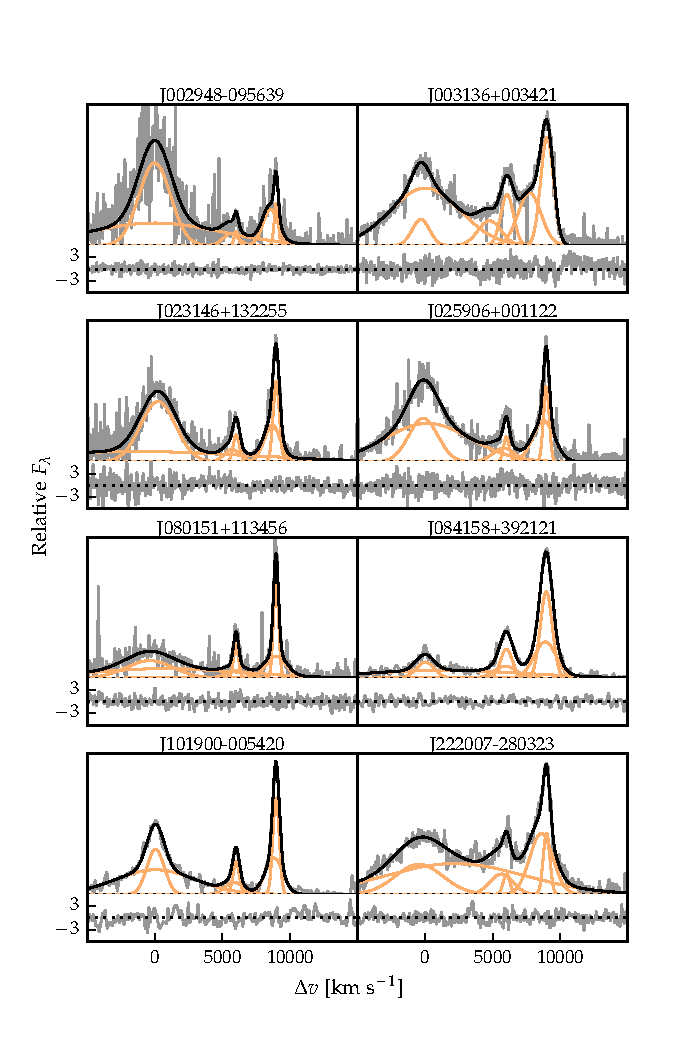
\includegraphics[width=\textwidth]{figures/chapter04/example_spectrum_grid.pdf} 
    \caption[{Model fits to the continuum- and \ion{Fe}{II}-subtracted \hbns/[\ion{O}{III}] emission in eight quasars, chosen at random.}]{Model fits to the continuum- and \ion{Fe}{II}-subtracted \hbns/[\ion{O}{III}] emission in $15$ quasars, chosen at random. The data is shown in grey, the best-fitting model in black, and the individual model components in orange. The peak of the [\ion{O}{III}] emission is used to set the redshift, and $\Delta{v}$ is the velocity shift from the rest-frame transition wavelength of \hb. Below each spectrum we plot the data minus model residuals, scaled by the errors on the fluxes.}     
    \label{fig:example_spectrum_grid}
\end{figure}

\subsection{Deriving emission-line properties from the best-fitting models}

\begin{table}
  \centering
  \footnotesize
  \caption{The format of the table containing the emission-line properties from our parametric model fits.}
  \label{tab:nlr-specmeasure}
  \centering
    \begin{tabular}{cccc} 
    \hline
    Column & Name & Units & Description \\ 
    \hline
    1 & UID & & Catalogue name \\
    2 & OIII\_V$5$ & \kms & [\ion{O}{III}] $v_{5}$ \\
    3 & OIII\_V$5$\_ERR & \kms & Uncertainty in $v_{5}$ \\
    4 & OIII\_V$10$ & \kms & [\ion{O}{III}] $v_{10}$ \\
    5 & OIII\_V$10$\_ERR & \kms & Uncertainty in $v_{10}$ \\
    6 & OIII\_V$25$ & \kms & [\ion{O}{III}] $v_{25}$ \\
    7 & OIII\_V$25$\_ERR & \kms & Uncertainty in $v_{25}$ \\
    8 & OIII\_V$50$ & \kms & [\ion{O}{III}] $v_{50}$ \\
    9 & OIII\_V$50$\_ERR & \kms & Uncertainty in $v_{50}$ \\
    10 & OIII\_V$75$ & \kms & [\ion{O}{III}] $v_{75}$ \\
    11 & OIII\_V$75$\_ERR & \kms & Uncertainty in $v_{75}$ \\
    12 & OIII\_V$90$ & \kms & [\ion{O}{III}] $v_{90}$ \\
    13 & OIII\_V$90$\_ERR & \kms & Uncertainty in $v_{90}$ \\
    14 & OIII\_V$95$ & \kms & [\ion{O}{III}] $v_{95}$ \\
    15 & OIII\_V$95$\_ERR & \kms & Uncertainty in $v_{95}$ \\
    16 & z\_OIII & & [\ion{O}{III}] redshift \\
    17 & z\_OIII\_ERR & & Uncertainty in [\ion{O}{III}] redshift \\
    18 & OIII\_W$50$ & \kms & [\ion{O}{III}] $w_{50}$ \\
    19 & OIII\_W$50$\_ERR & \kms & Uncertainty in [\ion{O}{III}] $w_{50}$  \\
    20 & OIII\_W$80$ & \kms & [\ion{O}{III}] $w_{80}$ \\
    21 & OIII\_W$80$\_ERR & \kms & Uncertainty in [\ion{O}{III}] $w_{50}$  \\
    22 & OIII\_W$90$ & \kms & [\ion{O}{III}] $w_{90}$ \\
    23 & OIII\_W$90$\_ERR & \kms & Uncertainty in [\ion{O}{III}] $w_{50}$  \\
    24 & OIII\_A & & [\ion{O}{III}] asymmetry \\
    25 & OIII\_A\_ERR & & Uncertainty in [\ion{O}{III}] asymmetry \\
    26 & OIII\_EQW & \AA & [\ion{O}{III}] EQW \\
    27 & OIII\_EQW\_ERR & \AA & Uncertainty in [\ion{O}{III}] EQW \\
    28 & OIII\_LUM & \ergs & [\ion{O}{III}] luminosity \\
    29 & OIII\_LUM\_ERR & \ergs & Uncertainty in [\ion{O}{III}] luminosity \\
    30 & EQW\_FE\_$4434$\_$4684$ & \AA & \ion{Fe}{II} EQW \\
    31 & EQW\_FE\_$4434$\_$4684$\_ERR & \AA & Uncertainty in \ion{Fe}{II} EQW \\
    32 & HB\_VPEAK & \kms & \hb peak velocity \\
    33 & HB\_VPEAK\_ERR & \kms & Uncertainty in \hb peak velocity \\
    34 & HA\_VPEAK & \kms & \ha peak velocity \\
    35 & HA\_VPEAK\_ERR & \kms & Uncertainty in \ha peak velocity \\
    36 & HB\_Z & & \hb redshift \\
    37 & HB\_Z\_ERR & & Uncertainty in \hb redshift \\
    38 & HA\_Z & & \ha redshift \\
    39 & HA\_Z\_ERR & & Uncertainty in \ha redshift \\
    41 & OIII\_FE\_FLAG & & Bad \ion{Fe}{II} subtraction \\
    42 & OIII\_EXTREM\_FLAG & & Extreme [\ion{O}{III}] emission \\
    \hline
    \end{tabular}
\end{table}

All [\ion{O}{III}] line properties are derived from the [\ion{O}{III}]\l$5008$ emission, but, as described above, the kinematics of [\ion{O}{III}]\l$4960$ are constrained to be identical in our fitting routine. 

We do not attach any physical meaning to the individual Gaussian components used in the model. 
Decomposing the [\ion{O}{III}] emission into a narrow component component at the systemic redshift and a lower-amplitude, blueshifted broad component is subject to large uncertainties and is highly dependent on the spectral S/N and resolution. 
Furthermore, there is no theoretical justification that the broad component should have a Gaussian profile.  

We therefore choose to characterize the [\ion{O}{III}] line profile using a number of non-parametric measures, which are commonly used in the literature \citep[e.g.][]{zakamska14,zakamska16}. 
A normalised cumulative velocity distribution is constructed from the best-fitting model, from which the velocities below which $5$, $10$, $25$, $50$, $75$, $90$, and $95$ per cent of the total flux accumulates can be calculated. 
These velocities are then adjusted so that the peak of the [\ion{O}{III}] emission is at 0\,\kms. 

The width of the emission-line can then be defined using either $w_{50}$ ($\equiv v_{75} - v_{25}$), $w_{80}$ ($\equiv v_{90} - v_{10}$) or $w_{90}$ ($\equiv v_{95} - v_{5}$). 
In terms of the FWHM, $w_{50} \simeq {\mathrm FWHM} / 1.746$, $w_{80} \simeq {\mathrm FWHM} / 0.919$, $w_{90} \simeq {\mathrm FWHM} / 0.716$, assuming a Gaussian line profile.  
$w_{90}$ is relatively more sensitive to the wings of the line profile, whereas $w_{50}$ is relatively more sensitive to the core.
We also define the relative asymmetry of the line as:

\begingroup\makeatletter\def\f@size{11}\check@mathfonts
\begin{eqnarray}
  A = \frac{(v_{90} - v_{\mathrm peak}) - (v_{\mathrm peak} - v_{10})}{(v_{90} - v_{10})}.     
\end{eqnarray} 
\endgroup

\noindent All of the derived parameters we have calculated are summarised in Table~\ref{tab:nlr-specmeasure}. 
The columns are as follows: 

\begin{itemize}

    
  \item[1] Unique ID: QSOXXX.

  \item[2-3] Systemic redshift measured at [\ion{O}{III}] peak wavelength, and its error. 

  \item[4-17] $v_{5}$, $v_{10}$, $v_{25}$, $v_{50}$, $v_{75}$, $v_{90}$ and $v_{95}$ velocity of [\ion{O}{III}], relative to [\ion{O}{III}] peak, and their errors, in \kms.  

  \item[18-23] $w_{50}$ ($\equiv v_{75} - v_{25}$), $w_{80}$ ($\equiv v_{90} - v_{10}$) and $w_{90}$ ($\equiv v_{95} - v_{5}$) velocity width of [\ion{O}{III}], and their errors, in \kms.

  \item[24-25] Dimensionless [\ion{O}{III}] asymmetry $A$, and its error.

  \item[26-27] Rest-frame [\ion{O}{III}] EQW, and its error, in \AA.

  \item[28-29] 1-$\sigma$ upper-limit on rest-frame [\ion{O}{III}] EQW, in \AA. %OIII\_5007\_EQW\_MEAN, OIII\_5007\_EQW\_STD

  \item[30-31] [\ion{O}{III}] luminosity, and its error, in \ergs. 

  \item[32-33] 4434-4684 \AA\, rest-frame \ion{Fe}{II} EQW, and its error, in \AA. % Not the same as used in EV1 plots 

  \item[34-35] Velocity of \hb peak, relative to [\ion{O}{III}] peak, in \kms, and its error. 

  \item[36-37] Velocity of \ha peak, relative to [\ion{O}{III}] peak, in \kms, and its error. 

  \item[38-38] Redshift of \hb peak, and its error.

  \item[40-41] Redshift of \ha peak, and its error.

  \item[44] \ion{Fe}{II} flag. 

  \item[45] Extreme [\ion{O}{III}] flag.   

  \item[46-47] \ion{C}{IV} $v_{50}$, relative to [\ion{O}{III}] peak, in \kms, and its error.

\end{itemize}

\subsection{Deriving uncertainties on parameters}

Our method to estimate realistic uncertainties on emission-line properties derived from the best-fitting model is very similar to the one described in Section~\ref{sec:ch3_param_errors}. 
Very briefly, random simulations of each spectrum are generated.
Our fitting-procedure is run on each simulated spectrum, and the errors on the line parameters are estimated by looking at the distribution of values from the ensemble of simulations. 
In a slight modification of the procedure in Section~\ref{sec:ch3_param_errors}, the error is defined as half the the $68$ ($84$ - $16$) percentile spread in the parameter values. 

\subsection{Low EQW [\ion{O}{III}]}

\begin{figure}
    \centering
    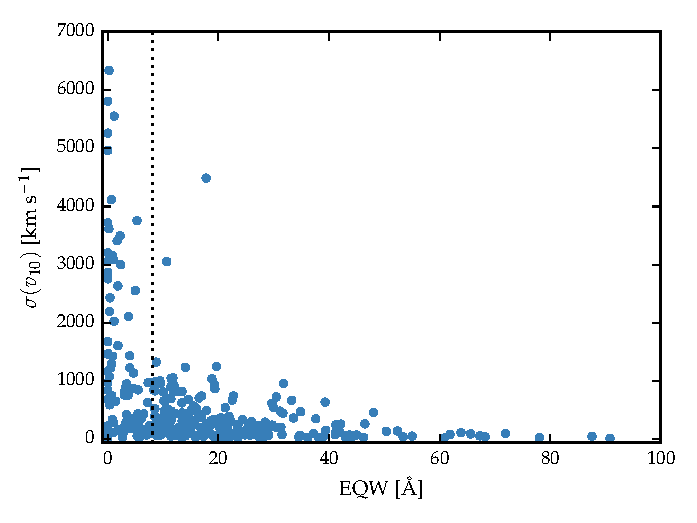
\includegraphics[width=0.8\textwidth]{figures/chapter04/eqw_cut.pdf} 
    \caption[{Uncertainty in $v_{10}$ as a function of the EQW, for [\ion{O}{III}].}]{Uncertainty in $v_{10}$ as a function of the EQW, for [\ion{O}{III}]. Uncertainties in $v_{10}$ are large to the left of the vertical line, at $8$\,\AA. These objects are ignored in our subsequent analysis of the [\ion{O}{III}] line shape.}     
    \label{fig:eqw_cut}
\end{figure}

In Figure~\ref{fig:eqw_cut} we show how the uncertainty in $v_{10}$ depends on the EQW. 
As the strength of [\ion{O}{III}] decreases, the average uncertainty in $v_{10}$ increases.
When the [\ion{O}{III}] ${\mathrm EQW} > 80$\,\AA, the mean uncertainty in $v_{10}$ is $50$\,\kms; this increases to $450$\,\kms\, when $10 < {\mathrm EQW} < 20$\,\AA. 
As the EQW drops below $8$\,\AA, typical uncertainties in $v_{10}$ become very large (exceeding $1000$\,\kms\, in many objects). 
Clearly, the emission-line is too weak for properties - in this case $v_{10}$ - to be reliably measured in many of these objects. 
Therefore, when the [\ion{O}{III}] line properties (e.g. velocity-width, centroid) are analysed in later sections, these objects with ${\mathrm EQW} < 8$\,\AA\, will be excluded. 
This leaves $226$ quasars in the sample. 

\subsection{Reliability of systemic redshift estimates}
\label{sec:ch4_redshifts}

\begin{figure}
   \captionsetup[subfigure]{labelformat=empty}
    \centering
    \subfloat[\label{fig:redshift_comparison_a}]{}
    \subfloat[\label{fig:redshift_comparison_b}]{}
    \subfloat[\label{fig:redshift_comparison_c}]{}
    \subfloat[]{{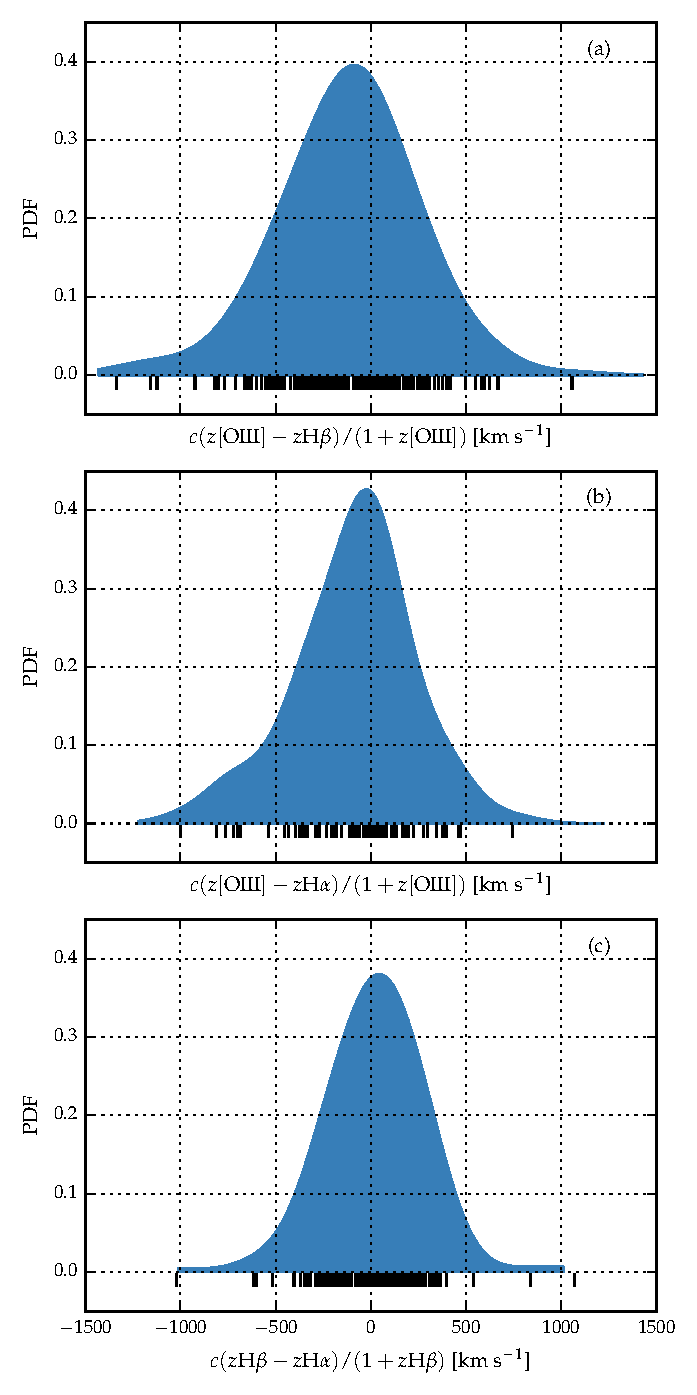
\includegraphics[width=0.8\linewidth]{figures/chapter04/redshift_comparison.pdf} }}
    \caption[{Comparison of systemic redshift estimates using [\ion{O}{III}], broad \hb and broad \hans.}]{Comparison of systemic redshift estimates using [\ion{O}{III}], broad \hb and broad \hans. The probability density functions are generated using a Gaussian kernel density estimator with a $\simeq150$\,\kms\, kernel width. The short black lines show the locations of the individual points.}       
    \label{fig:redshift_comparison}
\end{figure}

In this section, we compare systemic redshift estimates based on [\ion{O}{III}], \hb and \hans. 
The wavelength of each of these lines is measured at the peak of the emission and this measurement is made using the best-fitting parametric model. 
In the case of the Balmer lines, this model includes both broad and (if present) narrow emission features. 

We compare systemic redshift estimates based on [\ion{O}{III}] and \hb (Figure~\ref{fig:redshift_comparison_a}), [\ion{O}{III}] and \ha (Figure~\ref{fig:redshift_comparison_b}) and \hb and \ha (Figure~\ref{fig:redshift_comparison_c}). 
[\ion{O}{III}], \hb and \ha measurements are available for $226$, $418$ and $226$ objects respectively. 
We exclude [\ion{O}{III}], \hb and \ha measurements when the uncertainties on the peak velocities exceed $200$, $300$ and $200$\,\kms\, respectively. 
This excludes $4$, $6$ and $12$ per cent of the [\ion{O}{III}], \hb and \ha measurements respectively. 
We also exclude [\ion{O}{III}] measurements from 16 objects with very broad, blueshifted [\ion{O}{III}] emission that is strongly blended with the red wing of \hb (these objects are discussed in Section~\ref{sec:extreme_oiii}) because these redshifts are almost certainly strongly biased.
After these cuts, there are $182$, $85$ and $162$ objects being compared in samples (a), (b) and (c) respectively. 

We generate probability density functions using a Gaussian kernel density estimator.
The bandwidth, which is optimised using leave-one-out cross-validation, is $170$, $120$ and $140$\,\kms\, for samples (a), (b) and (c) respectively. 
The systematic offset between the \ha and \hb estimates is consistent with being zero, and the scatter is $230$\,\kms. 
The scatter in these distributions is consistent with previous studies of redshift uncertainties from broad emission-lines \citep[e.g.][]{shen16b}. 
The [\ion{O}{III}] redshifts appear to be systematically offset in comparison to both \ha and \hbns, in the sense that [\ion{O}{III}] is blueshifted. 
This effect is strongest when [\ion{O}{III}] is compared to \hbns, in which case [\ion{O}{III}] is shifted by $\sim100$\,\kms\, to the blue.

\citet{hewett10} found that [\ion{O}{III}] was blueshifted by $\sim45$\,\kms\, relative to a rest-frame defined using photospheric \ion{Ca}{II}\ll$3935$,$3970$ absorption in the host galaxies of $z<0.4$ SDSS AGN. 
They also noted, as we find here, that [\ion{O}{III}] is increasingly blue-asymmetric at higher luminosities. 
Therefore, our finding is consistent with \citet{hewett10}, when the very different luminosities of the two samples are accounted for.  

\section{Results}
\todo{Highlight key results more prominantly}

\begin{figure}
    \captionsetup[subfigure]{labelformat=empty}
    \centering
    \subfloat[\label{fig:parameter_hists_a}]{}
    \subfloat[\label{fig:parameter_hists_b}]{}
    \subfloat[\label{fig:parameter_hists_c}]{}
    \subfloat[]{{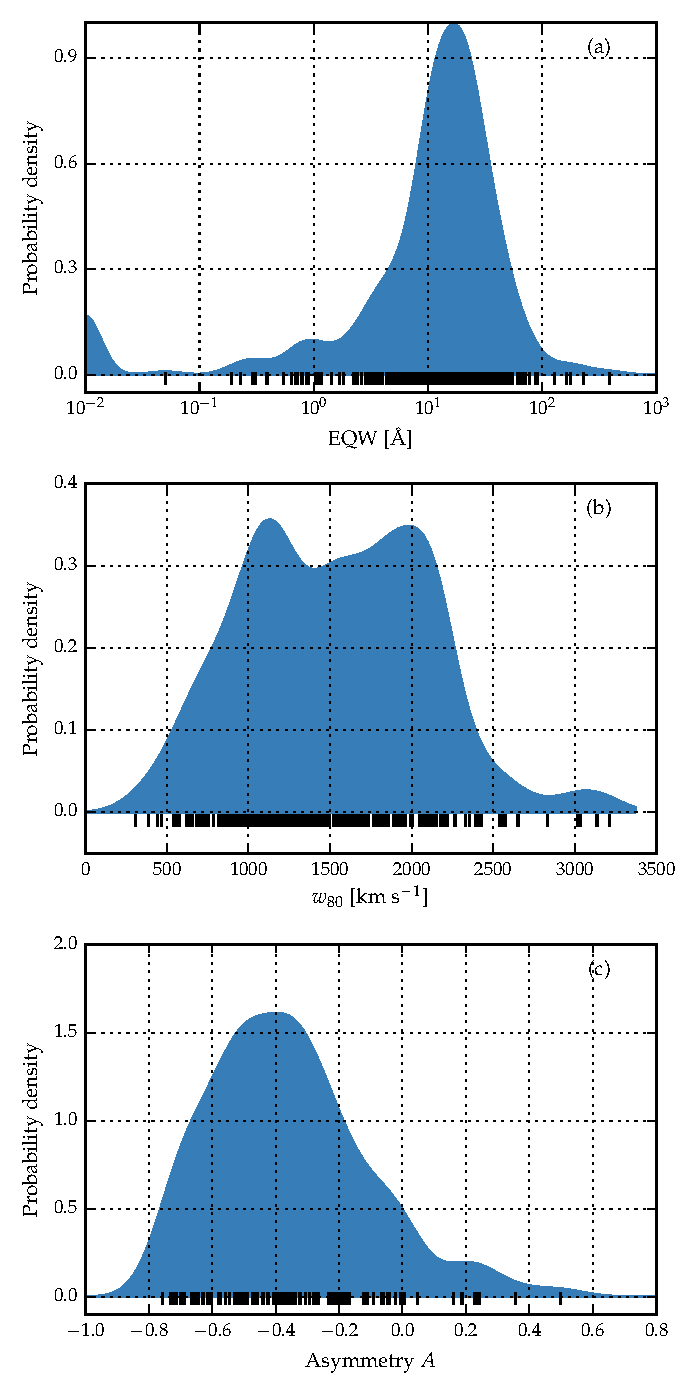
\includegraphics[width=0.8\columnwidth]{figures/chapter04/parameter_hists.pdf} }}
    \caption[{Probability density distributions of the [\ion{O}{III}] parameters EQW (a), $w_{80}$ (b) and asymmetry $R$ (c).}]{Probability density distributions of the [\ion{O}{III}] parameters EQW (a), $w_{80}$ (b) and asymmetry $R$ (c). The $1200$\,\kms\, upper limit on the velocity width of the Gaussian functions used to model [\ion{O}{III}] is responsible for the peak at $1200$\,\kms\, in (b).}     
    \label{fig:parameter_hists}
\end{figure}

In our sample of $354$ quasars, there is a huge diversity in [\ion{O}{III}] emission properties (Figure~\ref{fig:example_spectrum_grid}). 
In Figure~\ref{fig:parameter_hists}, we present a sub-set of the measurements we have made of the [\ion{O}{III}] line.  

The strength of [\ion{O}{III}] depends on the covering factor of NLR gas, its density and ionisation parameter. 
The [\ion{O}{III}] EQW follows an approximately log-normal distribution, peaking at $17$\,\AA. 
In $10$ per cent of our sample [\ion{O}{III}] is very weak, with ${\mathrm EQW} < 1$\,\AA.  
The average [\ion{O}{III}] strength is consistent with earlier studies on smaller samples \citep[e.g.][]{sulentic04,netzer04,shen16a}.

The mean and standard deviation of the line width (characterized by $w_{80}$) is $1535\pm562$\,\kms, with a median of $1529$, minimum of $206$ and maximum of $3214$. 
This is consistent with recent near-infrared spectroscopy of $z>1.5$ quasars which often report velocity widths $\gtrsim1000$\,\kms\, \citep[e.g.][]{netzer04,kim13,brusa15,shen16a}. 
For gas discs rotating in the potential of the massive galaxies line widths do not exceed $w_{80}\simeq600$\,\kms\, \citep{liu13}. 
Therefore the [\ion{O}{III}] gas cannot be in dynamical equilibrium with the host-galaxy. 
[\ion{O}{III}] emission is suppressed by collisional de-excitation in higher-density environments, and so the large velocity widths cannot be due to Doppler broadening in the BLR. 

The [\ion{O}{III}] asymmetry is shown in Figure~\ref{fig:parameter_hists_c}. 
In $40$ per cent of the sample [\ion{O}{III}] is fit with a single Gaussian. 
The asymmetry is zero in this model and so these objects are excluded. 
For the objects fit with two Gaussians, [\ion{O}{III}] is blue-asymmetric in 90 per cent. 
This indicates that there is an outflow component in the [\ion{O}{III}]-emitting gas. 
We also find a weak anti-correlation between $w_{80}$ and the asymmetry (Spearman correlation coefficient: $-0.30$, p-value:L $4e-4$), in the sense that the broaded lines tend to be more blue-asymmetric.  

\subsection{Luminosity/redshift-evolution of [\ion{O}{III}] properties}

We extend the dynamic range of our samples in terms of both luminosity and redshift by supplementing our sample with quasars presented by \citet{mullaney13} and \citet{harrison16}. 
The \citet{mullaney13} catalogue contains [\ion{O}{III}] line measurements for $\sim25\,000$ optically-selected AGN with SDSS spectra at $z<0.4$.
\citet{mullaney13} fit [\ion{O}{III}] with one or two Gaussians, and then used similar non-parametric measures to the ones we adopt.
We select only the Type I AGN from the \citet{mullaney13} catalogue. 
The \citet{harrison16} sample contains $40$ X-ray selected quasars ($L_{2-10 {\mathrm keV}} \simeq 10^{43-44}$\,\ergs) at intermediate redshifts ($1.1 < z < 1.7$) observed with the KMOS integral field unit spectograph on the VLT. 
We also use the SDSS DR$7$ quasar catalogue, with properties derived by \citet{shen11}. 
[\ion{O}{III}] is visible in SDSS spectra up to redshifts $z=0.84$. 
There are $20\,663$ quasars in the \citet{shen11} catalogue with [\ion{O}{III}] ${\mathrm EQW} > 0$\,\AA. 

\subsubsection{Equivalent width}

\begin{figure}[t!]
\centering 
    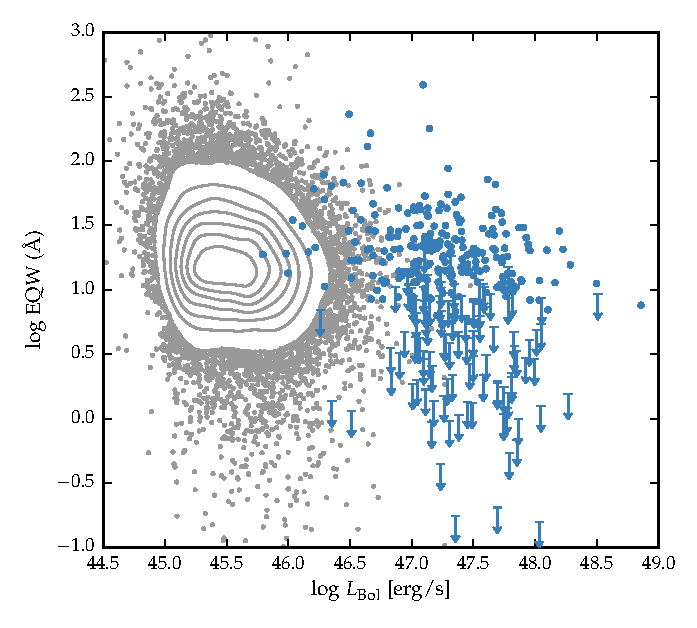
\includegraphics[width=\columnwidth]{figures/chapter04/eqw_lum.pdf} 
    \caption[{The [\ion{O}{III}] EQW as a function of the quasar bolometric luminosity for the sample presented in this chapter (blue circles) and the low-$z$ SDSS sample (grey points and contours).}]{The [\ion{O}{III}] EQW as a function of the quasar bolometric luminosity for the sample presented in this chapter (blue circles) and the low-$z$ SDSS sample (grey points and contours). An upper limit at ${\mathrm EQW}=1$\,\AA\, indicates points with ${\mathrm EQW} < 1$\,\AA. The red line shows the median [\ion{O}{III}] EQW in luminosity bins centred on $45.3$, $45.7$, $46.1$, $46.6$, $47.2$ and $47.7$\,\ergs, considering only objects with ${\mathrm EQW} > 1 $\,\AA.}     
    \label{fig:eqw_lum}
\end{figure}


\begin{figure}[t!]
    \centering 
    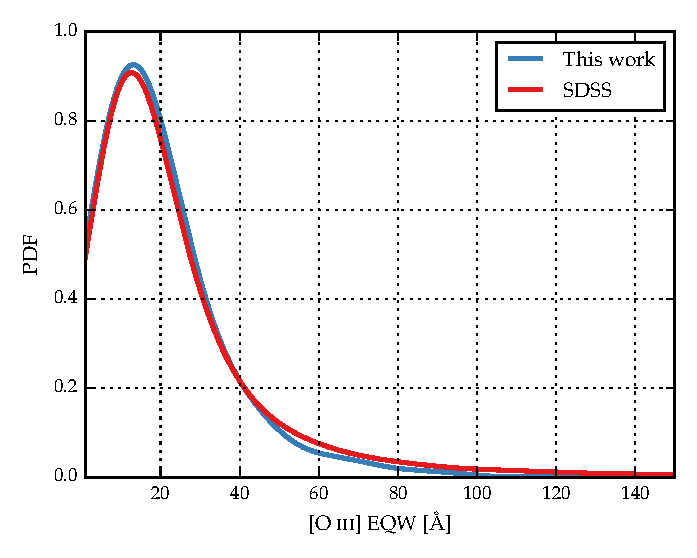
\includegraphics[width=\columnwidth]{figures/chapter04/high_eqw_comp.pdf} 
    \caption[{}]{[\ion{O}{III}] EQW distribution at ${\mathrm EQW} > 1 $\,\AA\, PDF generated using a Gaussian KDE with a $8$\,\AA\, bandwidth (optimized via leave-one-out cross-validation). The two distributions are essentially identical, and peak at $13$\,\AA. However, $10$ per cent of the sample in this work have ${\mathrm EQW} < 1$\,\AA, compared to just $1$ per cent of the SDSS sample.}     
    \label{fig:high_eqw_comp}
\end{figure}

In Figure~\ref{fig:eqw_lum} we show the [\ion{O}{III}] EQW as a function of the quasar bolometric luminosity. 
Bolometric luminosity is estimated from the monochromatic continuum luminosity at $5100$\,\AA, using the correction factor given by \citet{richards06}. 
For comparison, we also show the sample from \citet{shen11}.  

Many authors have reported the [\ion{O}{III}] EQW to decrease with quasar luminosity \citep[e.g.][]{brotherton96,sulentic04,baskin05b}. 
The origin of this correlation - which is known as the Baldwin effect \citep[e.g.][]{baldwin77,brotherton96,zhang11,stern12} - has not been demonstrated conclusively. 
One interpretation is that the size of the NLR increases when the quasar luminosity increases, because more ionising photons are available. 
However, beyond a certain radius there will be no more gas left to ionise, and the size of the NLR will plataeu.

We do not observe a Baldwin effect in our sample, despite the luminosity range spanning three dex. 
This is seen more clearly if we show the distribution of EQWs in the SDSS sample ($\log{\mathrm L_{Bol}} \sim 45.5$\,\ergs) and the sample presented in this paper ($\log{\mathrm L_{Bol}} \sim 47.3$\,\ergs).
Only objects where [\ion{O}{III}] is detected with ${\mathrm EQW} > 1$\,\AA\, are included.
The two distributions are essentially identical, and peak at $13$\,\AA. 

The fraction of objects with very weak [\ion{O}{III}] (${\mathrm EQW} < 1$\,\AA) is $10$ per cent in our sample, compared to one per cent of the SDSS sample. 
Therefore, the fraction of objects with very weak [\ion{O}{III}] is an order of magnitude larger in the more luminous sample. 
If we instead define `weak' [\ion{O}{III}] emission as having an ${\mathrm EQW} < 5$\,\AA, then $22$ per cent of our high-luminosity sample is classified as such, compared to $8$ per cent of the SDSS sample. 

\citet{netzer04}, comparing the [\ion{O}{III}] properties in a much smaller sample over a comparable luminosity range, reached a similar conclusion. 
The conclusion reached by \citet{netzer04} was that the size of the NLR scaled with the square root of the luminosity of the source of ionising photons in low luminosity AGN, in line with theoretical predictions \citep[e.g.][]{netzer90}. 
However, extrapolating this relationship to high luminosity quasars leads to the prediction of enormous NLRs with galactic dimensions. 
If these NLRs had properties similar to the ones in local Seyferts, they would quickly escape the system and disappear. 
Therefore, the prediction is that no NLR emission should be observed in high-luminosity quasars, which is the case for $\sim10$ per cent of our sample. 
This means that when strong [\ion{O}{III}] is detected, it must be from denser gas. 
\citet{netzer04} suggest that this high density gas could be produced in the kilo-parsec scale nuclear regions by violent star formation.  
We find that that virtually all objects which have large \ion{C}{IV} blueshifts have very weak [\ion{O}{III}] emission. 
\todo{Does this support/contradict Netzer picture? See email from Paul.}

% At very high luminosity the NLR becomes very large (e.g., Hainline et al. 2013; Zakamska et al. 2016). 
% In these conditions, the NLR size-luminosity relationship flattens out (Hainline et al. 2013, 2014), and the [O iii] luminosities may become saturated as the AGN photoionizes the entire interstellar medium of the host galaxy (e.g., Hainline et al. 2013). 
 
\subsection{Velocity width}

\begin{figure}[t!]
    \centering
    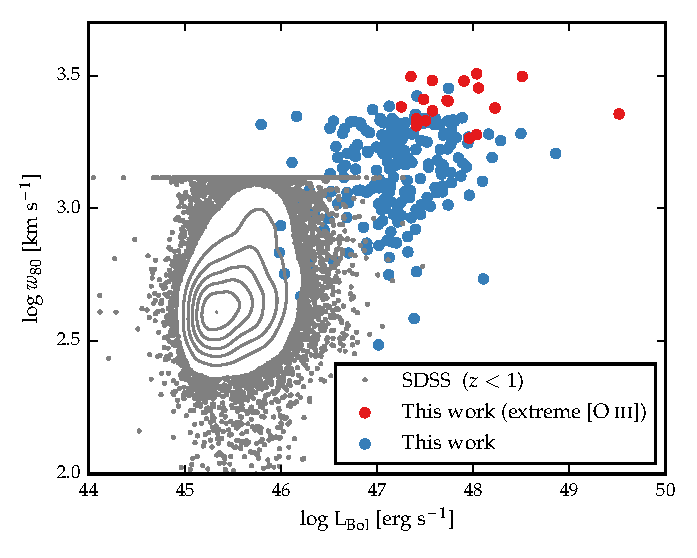
\includegraphics[width=\columnwidth]{figures/chapter04/lum_w80.pdf} 
    \caption[{}]{[\ion{O}{III}] velocity width $w_{80}$ as a function of quasar bolometric luminosity. Objects with extreme [\ion{O}{III}] profiles (Section~\ref{sec:extreme_oiii}) are shown in red.}     
    \label{fig:lum_w80}
\end{figure}

In Figure~\ref{fig:lum_w80} we show the [\ion{O}{III}] velocity width as a function of the quasar optical luminosity.
A strong correlation exists. 
On the other hand, we do not find any significant correlation between the [\ion{O}{III}] velocity width and the quasar redshift. 
The lack of any evolution in typical [\ion{O}{III}] properties between $z=0$ and $z=1.5$ has previously been reported \citep[e.g.][]{harrison16}; our sample demonstates that the [\ion{O}{III}] properties do not evolve from $z=1.5$ all the way to $z=4$. 

\section{Eigenvector 1 correlations}

\subsection{EV1 trends exist in high-redshift quasars}

\begin{figure}[t!]
\centering 
    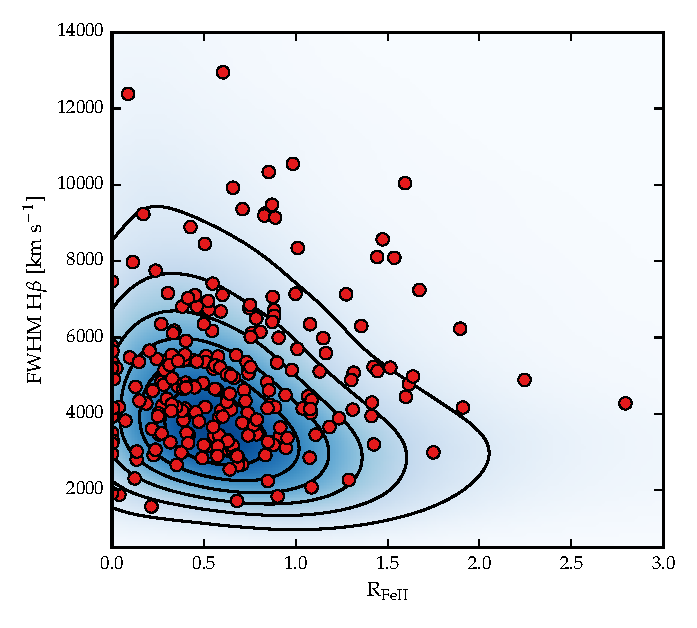
\includegraphics[width=\columnwidth]{figures/chapter04/ev1_lowz.pdf} 
    \caption[{EV1 parameter space.}]{EV1 parameter space. The contours and shading show low-redshift, low-luminosity SDSS AGN (with measurements taken from \citealt{shen11}) and the red circles show the high-redshift, high-luminosity objects presented in this chapter.}      
    \label{fig:ev1_lowz}
\end{figure}

\begin{figure}[t!]
\centering 
    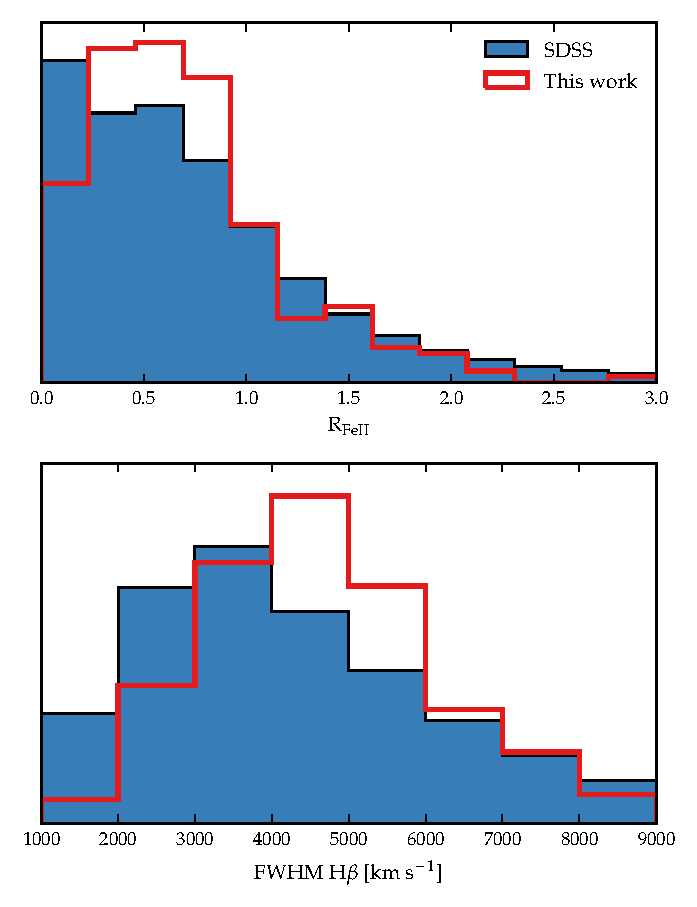
\includegraphics[width=\columnwidth]{figures/chapter04/ev1_hists.pdf} 
    \caption[{}]{EV$1$ parameters for the high-luminosity quasar sample presented in this work and the low-luminosity SDSS sample. \hb FWHM are shifted to higher values in the high-luminosity sample, which is consistent with these quasars having large BH masses. The \ion{Fe}{II} distributions are similar.}      
    \label{fig:ev1_hists}
\end{figure}


The FWHM of the broad \hb emission-line and the strength of [\ion{O}{III}] and the relative strengths of optical \ion{Fe}{II} and \hb have been identified as the features responsible for the largest variance in the spectra of AGN.
These parameters form part of EV$1$, the first eigenvector in a PCA which originated from the work of \citet{boroson92}.   
The underlying driver behind EV$1$ is thought to be the Eddington ratio \citep[e.g.][]{sulentic00b,shen14}.

In Figure~\ref{fig:ev1_lowz} we show the [\ion{O}{III}] EQW as a function of the \hb FWHM and the optical \ion{Fe}{II} strength. 
The optical \ion{Fe}{II} strength is defined as the ratio of the \ion{Fe}{II} and \hb EQW, where the \ion{Fe}{II} EQW is measured between $4434$ and $4684$\,\AA.
There are $395$ objects in our sample with spectra covering \hb. 
$303$ with partial ($>150$\,\AA) coverage of the $4434$-$4684$ region to constrain the \ion{Fe}{II} emission.
$283$ after removing bad fit \ion{Fe}{II}. 
$230$ excluding those with more than $25$ per cent fractional error in \hb FHWM or \ion{Fe}{II} strength. 

The low-redshift SDSS sample, with parameters taken from \citet{shen11}, is also shown in Figure~\ref{fig:ev1_lowz}.
In our sample, these parameters follow very similar correlations to what is observed at low-redshift.
In particular, we observe a strong anti-correlation between the [\ion{O}{III}] and \ion{Fe}{II} EQW.  
The \hb FWHM are displaced to higher values, which is consistent with the high-redshift, high-luminosity sample having larger BH masses. 
Thus, we confirm earlier results using much smaller samples that suggest that the same EV$1$ correlations exist in high-redshift quasars \citep[e.g.][]{netzer04,sulentic04,sulentic06,runnoe13,shen16a}.

\subsection{Connecting EV1 at low and high redshifts}
\label{sec:ch4_low_high_ev1}

The \ion{C}{IV} blueshift and EQW is a diagnostic that similarly spans the diversity of broad emission-line properties in high redshift quasars \citep{sulentic07,richards11}. 
The similarity of the \ion{C}{IV} EQW-blueshift parameter space at high redshift to EV$1$ parameter space at low redshift suggests that these trends are connected. 
Because we have optical and near-infrared spectra for XX quasars in our sample, we are able to test how the low-redshift EV$1$ parameter space maps to the high-redshift \ion{C}{IV} parameter space.
In Figure~\ref{fig:ev1} we show how the EV$1$ parameters change as a function of position in the \ion{C}{IV} EQW-blueshift parameter space.

\begin{figure}
\centering 
    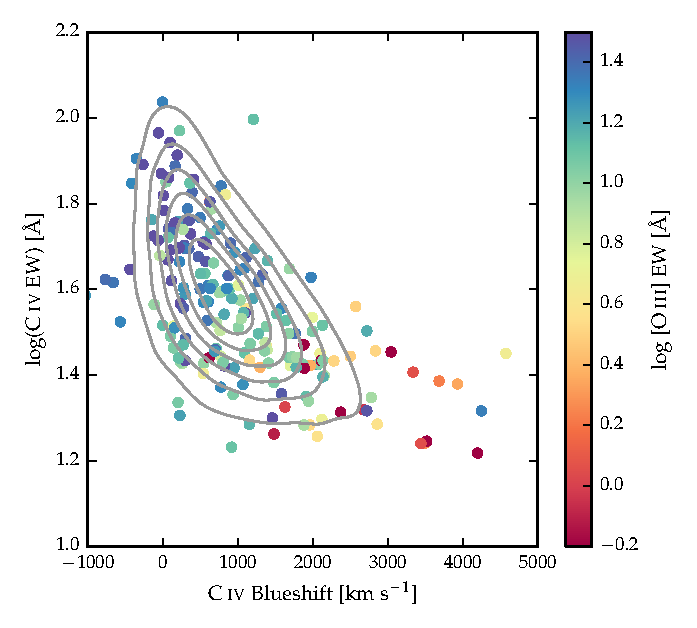
\includegraphics[width=\columnwidth]{figures/chapter04/ev1.pdf} 
    \caption[{The high-redshift EV$1$ parameter space of \ion{C}{IV} blueshift and EQW.}]{The high-redshift EV$1$ parameter space of \ion{C}{IV} blueshift and EQW. Our sample is shown with points, and quasars from the full SDSS catalogue are shown with grey contours. The [\ion{O}{III}] EQW varies systematically with position in the \ion{C}{IV} blueshift-EQW parameter space (a) but the \hb FWHM shows significantly less systematic variation (b).}      
    \label{fig:ev1}
\end{figure}

Two hundred and thirteen objects are shown in Figure~\ref{fig:ev1}.
Objects for which the \ion{C}{IV} line properties could not be measured reliably (see Section~\ref{sec:flagged_spectra}) have been removed. 
We consider only objects for which the \ion{C}{IV} EQW exceeds $15$\,\AA. 
The \ion{C}{IV} blueshift is measured relative to the redshift determined from the peak of [\ion{O}{III}], \hb or \hans. 
We also show the \ion{C}{IV} line parameters of $32\,157$ SDSS DR$7$ quasars at redshifts $1.6 < z < 3.0$. 
The derivation of the \ion{C}{IV} emission properties of these objects is described in Section XX. 

Most of the diversity in \ion{C}{IV} properties is correlated with the [\ion{O}{III}] EQW. 
This is seen more clearly in Figure~\ref{fig:civ_blueshift_oiii_eqw}, in which we plot the [\ion{O}{III}] EQW as a function of the \ion{C}{IV} blueshift. 
The correlation see in Figure~\ref{fig:civ_blueshift_oiii_eqw} is very strong. 
The mean [\ion{O}{III}] EQW is $40$\,\AA\, amongst the population of quasars with \ion{C}{IV} blueshifts $<500$\,\kms, compared to $5$\,\AA\, for quasars with \ion{C}{IV} blueshifts $>2000$\,\kms. 
In other words, the NLR emission appears to be missing in quasars with large \ion{C}{IV} blueshifts. 
One possibility is that the NLR gas is swept away on relatively short timescales by quasar outflows; this possibility is explored in more detail in Section XX. 

On the other hand, the \ion{C}{IV} blueshift and EQW cannot be used to predict the \hb FWHM. 
This is consistent with what we found in Chapter~\ref{ch:bhmass}: objects with large \ion{C}{IV} blueshifts have narrow Balmer emission-lines, but objects with modest \ion{C}{IV} blueshifts have a wide range of Balmer line widths. 

\begin{figure}
    \centering
    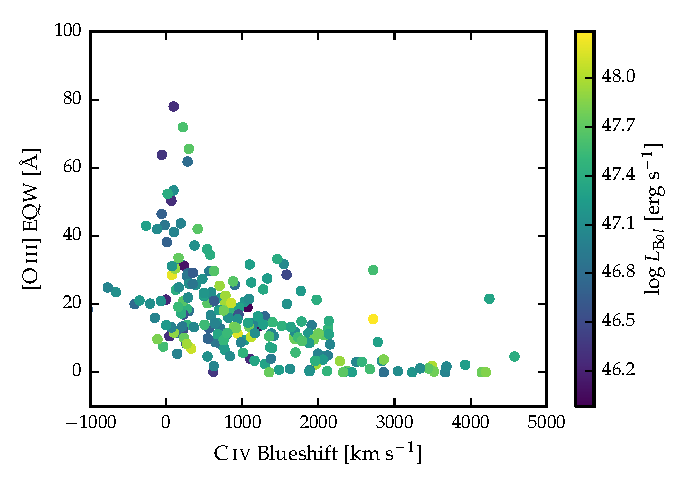
\includegraphics[width=\columnwidth]{figures/chapter04/civ_blueshift_oiii_eqw.pdf} 
    \caption[{[\ion{O}{III}] EQW as a function of the \ion{C}{IV} blueshift.}]{[\ion{O}{III}] EQW as a function of the \ion{C}{IV} blueshift. The [\ion{O}{III}] EQW is strongly anti-correlated with the \ion{C}{IV} blueshift. On the other hand, no strong luminosity-dependent trends (indicated by the colours of the points) is evident.}     
    \label{fig:civ_blueshift_oiii_eqw}
\end{figure}

\section{Extreme [\ion{O}{III}] emitters}
\label{sec:extreme_oiii}

\begin{figure}
    \centering
    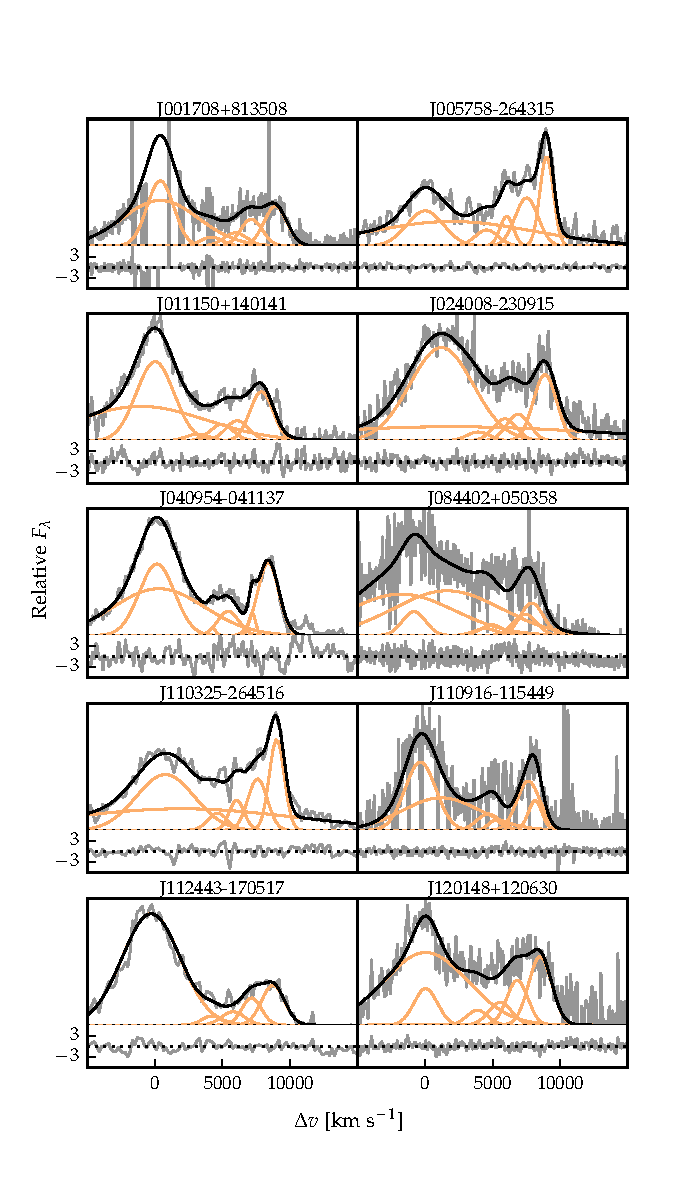
\includegraphics[width=\columnwidth]{figures/chapter04/example_spectrum_grid_extreme_oiii_1.pdf} 
    \caption[{Model fits to the continuum- and \ion{Fe}{II}-subtracted \hbns/[\ion{O}{III}] emission in $18$ quasars with extreme [\ion{O}{III}] emission profiles.}]{Model fits to the continuum- and \ion{Fe}{II}-subtracted \hbns/[\ion{O}{III}] emission in $18$ quasars with extreme [\ion{O}{III}] emission profiles. The data is shown in grey, the best-fitting model in black, and the individual model components in orange. The peak of the [\ion{O}{III}] emission is used to set the redshift, and $\Delta{v}$ is the velocity shift from the rest-frame transition wavelength of \hbns. Below each spectrum we plot the data minus model residuals, scaled by the errors on the fluxes.}     
    \label{fig:example_spectrum_grid_extreme_oiii}
\end{figure}

\begin{figure}
\ContinuedFloat
    \centering
    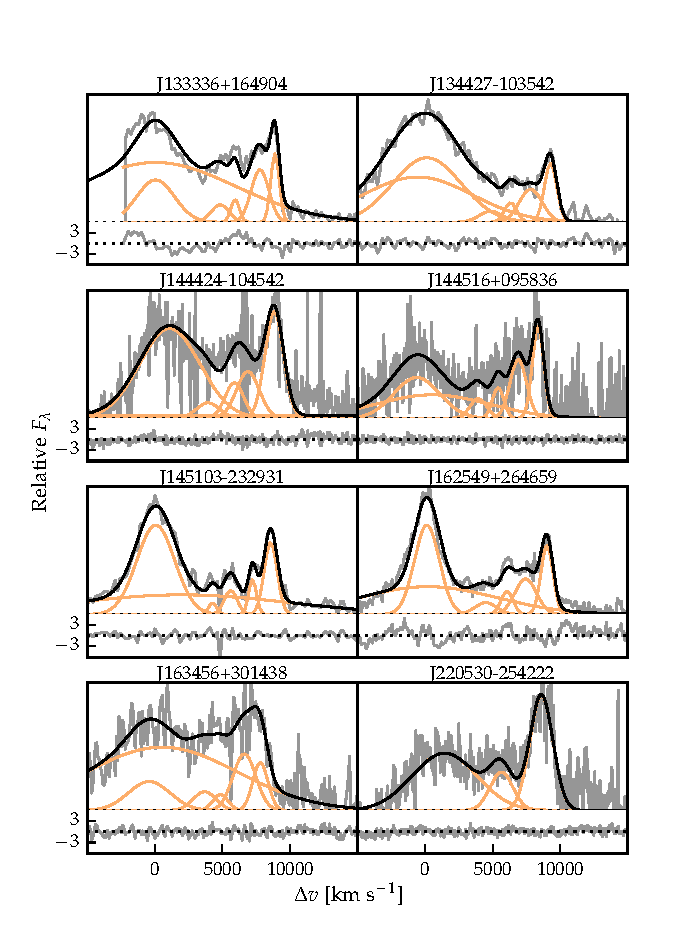
\includegraphics[width=\columnwidth]{figures/chapter04/example_spectrum_grid_extreme_oiii_2.pdf} 
    \caption[]{Continued.}     
\end{figure}

Figure~\ref{fig:example_spectrum_grid_extreme_oiii} shows the spectra of $18$ objects which we visually identified as having broad, blueshifted [\ion{O}{III}] emission which is heavily blended with the red wing of \hbns. 
Because the emission is so heavily-blended, it is difficult to determine unambiguously what combination of \hb, [\ion{O}{III}] and \ion{Fe}{II} is responsible for the unusual plateau-like emission observed in these objects. 
Therefore, uncertainties on the [\ion{O}{III}] emission properties are generally high in these objects. 

In Figure~\ref{fig:lum_w80} we show that the luminosities of all of these objects are larger than the sample median.
The mean luminosity of the quasars with extreme [\ion{O}{III}] emission is $10^{47.9}$\,\ergs, compared to $10^{47.2}$\,\ergs for the rest of the sample. 
Figure~\ref{fig:lum_w80} demonstrates that these quasars occupy a unique region of the $w_{80}$-L$_{\mathrm Bol}$ parameter space: $w_{80}\gtrsim1500$\,\kms\, and L$_{\mathrm Bol}\gtrsim10^{47.5}$\,\ergs. 

A similar [\ion{O}{III}] emission was also observed in J$1201$+$1206$ in a sample of five quasars at redshifts $2.3 \lesssim z \lesssim 3.5$ with luminosities $10^{47.5} < {\mathrm L_{Bol}} < 10^{48}$\,\ergs observed by \citet{bischetti16}.
These [\ion{O}{III}] emission-lines are also somewhat similar to the lines observed in a sample of four extremely dust-reddened quasars at $z\sim2$ recently identified by \citet{zakamska16}. 
The four \citet{zakamska16} quasars have $5$\,$\mu$m luminosities of $\sim10^{47}$\,\ergs, which is comparable to the $5$\,$\mu$m luminosities of the brightest objects in our sample. 
However, the [\ion{O}{III}] velocity widths of the \citet{zakamska16} objects are extreme in relation to our sample ($w_{80} \simeq 3500-5500$\,\kms). 
The extreme nature of the [\ion{O}{III}] emission in these objects led \citet{zakamska16} to propose that these objects are being observed transitioning from a dust-obscured, star-burst phase to a luminous, blue quasar \citep[e.g.][]{sanders88}.
Punctuated fuelling episodes, e.g. driven by galaxy mergers, satellite accretion and even secular processes,
almost certainly lead to AGN experiencing activity-, outflow- and obscuration-dominated cycles with some overlap between phases. 
This suggests that these extreme outflows signatures are only associated with rare/short-lived phases in the AGN cycle represented by the reddened quasars and are not ubiquitous in the luminous AGN population.
The early phase of feedback is likely to highly obscured by dusty inflowing material \citep[e.g.][]{haas03}.
Quasar-driven outflows will eventually blow away the obscuring dust, revealing a luminous, relatively un-obscured quasars.  
The fact that we do not see such extreme outflow signatures in our sample, where the mean dust reddening is just $0.03$, appears to support this idea.     

\subsection{Connections between [\ion{O}{III}] and \ion{C}{IV} outflows}

\begin{figure}
\centering 
    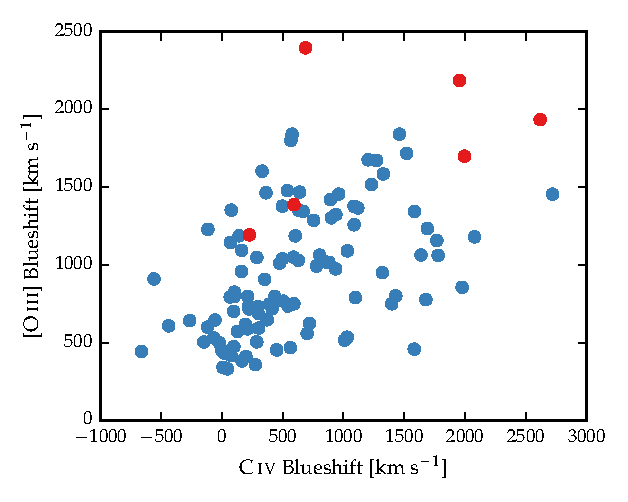
\includegraphics[width=\columnwidth]{figures/chapter04/civ_blueshift_oiii_blueshift.pdf} 
    \caption[{The relation between the blueshifts of \ion{C}{IV} and [\ion{O}{III}].}]{The relation between the blueshifts of \ion{C}{IV} and [\ion{O}{III}].}     
    \label{fig:oiii_civ_blueshifts}
\end{figure}

In Chapter~\ref{ch:bhmass} we found that \ion{C}{IV} is blueshifted realtive to the systemic redshift in a large majority of luminous, high-redshift quasars. 
In a sub-set, the blueshifting of \ion{C}{IV} can reach many thousands of \kms. 
This is strong evidence that quasars are capable of driving fast outflows, at least over the sub-parsec scale of the BLR. 
In the present chapter, we have found that outflows in the NLR, as indicated by broad velocity-widths and asymmetries in [\ion{O}{III}], are similarly ubiquitous in the luminous quasar population. 

In Section~\ref{sec:ch4_low_high_ev1}, we found that the [\ion{O}{III}] EQW has a very strong dependence on the \ion{C}{IV} blueshift.
The mean [\ion{O}{III}] EQW is $40$\,\AA\, amongst the population of quasars with \ion{C}{IV} blueshifts $<500$\,\kms, compared to $5$\,\AA\, for quasars with \ion{C}{IV} blueshifts $>2000$\,\kms. 
This establishes a connection between gas in the broad and narrow line regions. 

In Figure~\ref{fig:oiii_civ_blueshifts} we show the the [\ion{O}{III}] blueshift as a function of the \ion{C}{IV} blueshift, for the objects where [\ion{O}{III}] is detected with EQW$>8$\,\AA. 
The [\ion{O}{III}] blueshift is defined as $v_{10}$([\ion{O}{III}]) - $v_{\mathrm peak}$([\ion{O}{III}]) whereas the \ion{C}{IV} blueshift is defined as $v_{50}$(\ion{C}{IV}) - $v_{\mathrm peak}$([\ion{O}{III}]) with the \ion{C}{IV} line measurements taken from Chapter~\ref{ch:bhmass}.
We do not show objects for which the errors on the [\ion{O}{III}] and \ion{C}{IV} blueshifts exceed $250$ or $125$\,\kms\, respectively. 
These objects, shown in the top two panels of Figure~\ref{fig:oiii_civ_blueshifts}, have a similar dyamic range to the main sample, meaning our results should not be biased by their exclusion.  
We also remove the objects with extreme [\ion{O}{III}] emission, because the systemic redshift determined from the peak of the [\ion{O}{III}] emission is strongly biased in these objects. 

Because of the strong anti-correlation between the \ion{C}{IV} blueshift and the [\ion{O}{III}] EQW, removing objects with weak [\ion{O}{III}] eliminates most of the objects with large ($>2000$\,\kms) \ion{C}{IV} blueshifts.  
Nevertheless, [\ion{O}{III}] appears to be more blueshifted in quasars with large \ion{C}{IV} blueshifts.
Although the scatter is large, the correlation appears to be significant (Spearman correlation coefficient: $0.46$, $p$-value: $6e\text{-}7$). 
This suggests a direct connection between the gas kinematics in the broad and narrow line regions. 

We considered a number of of alternative approaches to parametrising both the [\ion{O}{III}] line shape and the systemic redshift. 
As expected, very similar trends are observed when the [\ion{O}{III}] line shape is parametrised using $v_{25} - v_{\mathrm peak}$, $v_{50} - v_{\mathrm peak}$, $w_{80} = v_{90} - v_{10}$, or the relative asymmetry $R$.
The same trend is also observed when the systemic redshift is defined using the peak of the \hb emission. 

The blueshifting of \ion{C}{IV} is known to correlate with luminosity \citep{richards11}.
In [\ion{O}{III}], the blueshifted wing becomes relatively more prominent as the luminosity of the quasar increases \citep{shen14}. 
Therefore, it is plausible that the correlation between the \ion{C}{IV} and [\ion{O}{III}] blueshifts is a secondary effect that is driven by the correlation of each with the luminosity. 
However, no strong luminosity-dependent trends are apparent in Figure~\ref{fig:oiii_civ_blueshifts}. 

\section{Discussion}

\subsection{Static NLR is removed by outflows}

Is the AGN NLR absent in objects where outflows have reached kilo-parsec scales, sweeping up the low-density material responsible for the [\ion{O}{III}]-emission?
If the BLR outflows can escape, they are very fast and wouldn't need long to clear out the NLR gas. 
Estimate a time-scale for how long the NLR would take to be cleared given typical size of galaxy and velocity of outflow. 

READ ZAKAMSKA DISCUSSION

It has been known for some time that the [\ion{O}{III}] EQW is anti-correlated with the strength of optical \ion{Fe}{II}, and this trend is thought to be driven by the Eddington ratio. 
\citet{shen14} showed that the amplitude of the core [\ion{O}{III}] emission decreases faster than the wing component as the Eddington ratio increases. 
Therefore, the [\ion{O}{III}] emission is weaker and more blueshifted in high accretion rate quasars.  
In Chapter~\ref{ch:bhmass} we found that all quasars with strong BLR outflows have high Eddington ratios. 
In this Section, we show that the \ion{C}{IV} and [\ion{O}{III}] blueshifts are directly linked. 
This suggests a direct connection between the gas kinematics in the broad and narrow line regions. 
But we need IFU to find out where this gas is (\todoinline{See text in research proposal}). 


\section{Independent Component Analysis}

\todoinline{Take out any results / discussion from this section and move to Gaussians. I don't think I learn anything with the ICA components I don't already know. }

\todoinline{ICA better with S/N - can give some examples from PCA work (ask Paul for references). If the [\ion{O}{III}] emission is confined to a relatively small number of components can then recover emission. Can show problem with $w_{80}$ as an example. Encouraging, but we do need a better training set (training set doesn't span the diversity of properties we see in the high-luminosity sample).}
\todoinline{The content of the ICA "test" is fine but I would suggest setting up the experiment somewhat differently and orienting the reader at the start. For example I would mention a) the likely lack of sensitivity to S/N [cf standard approach], b) equating components with physical properties of interest and thus potential effectiveness of component weights (e.g. what is to come in Fig. 1.16). Would also though put in the information about using the SDSS objects to generate the component set and how one probably expects the high-luminosity sample to include spectral diversity not present in the SDSS-sample [and hence in the ICA components]. You can, as you have drafted, then say how the analysis could be improved - better training set, removing the component cross-talk (I can tell you how this can be achieved),\dots}


In this section, we consider an alternative approach to the analysis presented in the bulk of this chapter. 
We use an independent component analysis (ICA) to separate the spectrum into a linear combination of statistically independent sub-components. 
Each individual spectrum can then be reconstructed with a linear combination of these components. 
The goal of this section is to determine whether or not the relative weights of the different components can be used in place of more commonly used emission-line parameters to understand the physical processes occurring in these quasars. 

Issues with the parametric model fitting approach adopted above include sensitivity to S/N. 
We also found the empirical template to be a poor match to the \ion{Fe}{II} emission observed in a number of quasars. 

\subsection{The technique}
 
ICA is a blind source separation technique for separating a signal into linearly mixed statistically independent subcomponents. 
Unlike the more widely-used principle component analysis technique, ICA produces non-negative components which allows for a physical interpretation of the components and weights.  
ICA has been successfully applied to model the spectra of emission-line galaxies \citep{allen13}. 
The quasar spectra can be thought of as a set of observations, $\bm{x}$, which are made up of statistically independent components, $\bm{c}$, that are combined by some mixing matrix, $\bm{W}$:

\begingroup\makeatletter\def\f@size{11}\check@mathfonts
\begin{eqnarray}
    \bm{x} = \bm{W}\bm{c}
\end{eqnarray}
\endgroup

\noindent ICA reverses this process and describes how the observed data are generated. 
Both the independent components and the mixing matrix are unknown, but can be found by solving:

\begingroup\makeatletter\def\f@size{11}\check@mathfonts
\begin{eqnarray}
    \bm{c} = \bm{W}^{-1}\bm{x}.
\end{eqnarray}
\endgroup

\noindent The components were solved for using a sample of $2,154$ SDSS quasars at redshifts XX. 
\todo{Ask Paul for details.}
At these redshifts the SDSS spectrograph covers the rest-frame region XX-XX\,\AA\, where \hb and [\ion{O}{III}] lie. 
The individual spectra were first adjusted to give the same overall shape as a model quasar template spectrum.
Six positive independent components and four lower-amplitude `correction' components that could be negative were found to be sufficient to reconstruct the spectrum, without over-fitting. 
Each quasar spectrum $x_j$ can then be represented as a linear combination of the independent components: 

\begingroup\makeatletter\def\f@size{11}\check@mathfonts
\begin{eqnarray}
    x_j = \sum_{i=1}^{10} c_{ij}W_{ij}
\end{eqnarray}
\endgroup

\subsubsection{Fitting procedure}

Each of the individual ICA components has been adjusted to give the same overall shape as a quasar template spectrum. 
We approximate the overall shape of this template by fitting a single power-law to emission-line free windows at $4200$-$4230$, $4435$-$4700$ and $5100$-$5535$\,\AA. 
We then flatten each of the ICA components by dividing by this power-law. 
An identical process is performed on each spectrum we fit, so that both the components and the spectrum to be fitted have essentially zero large-scale slope. 
For each quasar in our sample we perform a variance-weighted least-squares minimisation to determine the optimum value of the components weights.
The first six component weights are constrained to be non-negative, and the fit is performed in logarithmic wavelength space, so that each pixel corresponds to a fixed velocity width.   
The relative shift of the ICA components is also allowed to vary in the optimisation procedure, to account for errors in the systemic redshifts used to transform the spectra into rest-frame wavelengths. 

\subsection{Quality of fits}

In general, the ICA components are able to reconstruct the spectra of the objects in our sample. 
\todo{Need something more quantative Look at chi-squared distribution? Doesn't seem that reliable.}
We also find that that in some cases, the ICA reconstructions are superior at modelling the \ion{Fe}{II} emission than the \citet{boroson92} template. 

\subsection{Physical interpretation of ICA components}

\begin{figure}[t!]
    \centering
    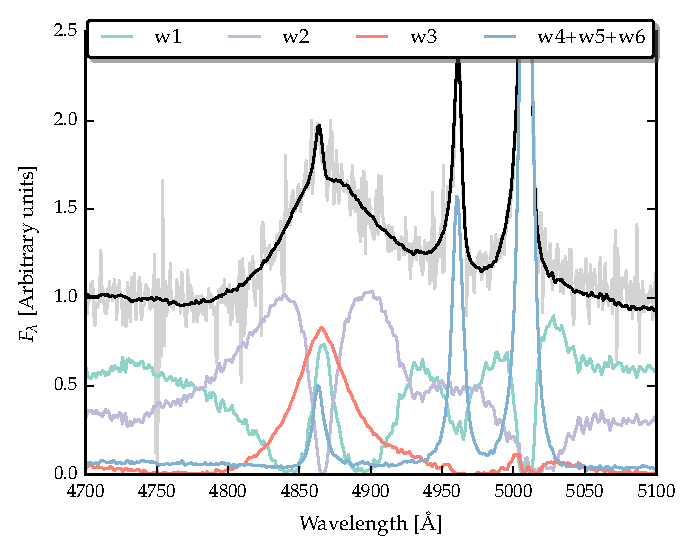
\includegraphics[width=0.8\textwidth]{figures/chapter04/mfica_components.pdf} 
    \caption{\hbns/[\ion{O}{III}] emission J$002952$+$020607$. The ICA reconstruction is shown in black, and the spectrum in grey. The first three components, and the sum of components four, five and six are shown individually.}     
    \label{fig:mfica_components}
\end{figure}

Although the ICA analysis is not based on any physics,  there appears to be a direct correspondence between the individual non-negative components and the different emission features which contribute to the spectra (Figure~\ref{fig:mfica_components}). 
This correspondence is summarised in Table~\ref{tab:icacomps}. 
The component $w_1$ seems to correspond to \ion{Fe}{II} emission, the components $w_2$ and $w_3$ to broad \hb emission, the components $w_4$ and $w_5$ to narrow [\ion{O}{III}] emission at the systemic redshift, and the component $w_6$ to broad, blueshifted [\ion{O}{III}] emission. 
s
\begin{table}[t!]
  \centering
  \footnotesize 
  \caption{Physical interpretation of the ICA components.}
  \label{tab:icacomps}
    \begin{tabular}{cc} 
    \hline
    Component & Origin \\
    \hline
    $w_1$& \ion{Fe}{II} \\
    $w_2$& \hbns \\
    $w_3$& \hbns \\
    $w_4$& [\ion{O}{III}] core \\
    $w_5$& [\ion{O}{III}] core \\
    $w_6$& [\ion{O}{III}] wing \\
    \hline
    \end{tabular}
\end{table} 

\subsubsection{Reconstructing the [\ion{O}{III}] profile}

\begin{figure}
    \centering
    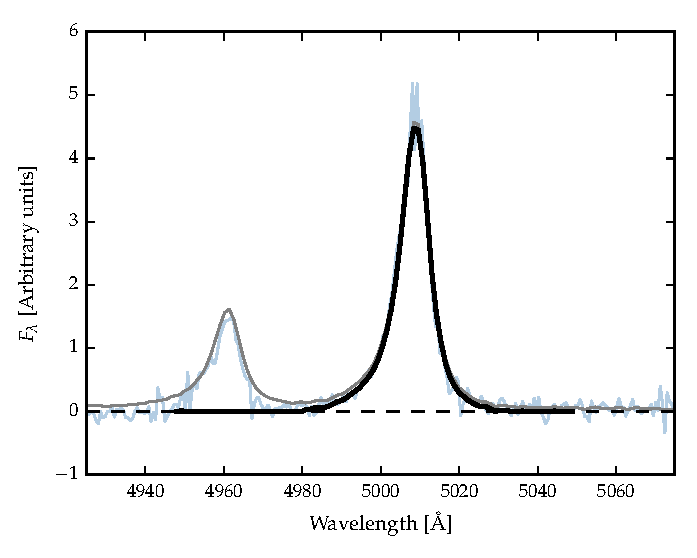
\includegraphics[width=0.8\textwidth]{figures/chapter04/oiii_reconstruction.pdf} 
    \caption[{[\ion{O}{III}] emission in J$002952$+$020607$.}]{[\ion{O}{III}] emission in J$002952$+$020607$. The data is shown in blue, and the ICA spectrum in grey. The first three ICA components have been subtracted from both the ICA composite and the data. The black curve shows the reconstructed [\ion{O}{III}]\l$5008$ profile.}     
    \label{fig:oiii_reconstruction}
\end{figure}

In order to measure non-parametric line parameters, e.g. $v_{10}$, we must first reconstruct the [\ion{O}{III}] emission. 
It is fortunate that most of the [\ion{O}{III}] emission is in just three of the ICA components; the remaining three contribute very little. 
Therefore, we can set the first three weights to zero to leave only the [\ion{O}{III}] emission. 
The four correction components are also included. 

We define the boundaries of [\ion{O}{III}]\l$5008$ as being between $4950$ and $5500$\,\AA. 
The blue limit is close to the peak of the [\ion{O}{III}]\l$4960$ line, and so to recover the intrinsic profile we instead use the blue wing of [\ion{O}{III}]\l$4960$. 
We use the emission from $4980$-$5050$\,\AA, and from $4900$-($4980$-($5008.2$-$4960.3$)). 
The blue window is then shifted by ($5008.2-4960.3$) to reconstruct the blue wing of the [\ion{O}{III}]\l$5008$ line. 
We then subtract a constant, because the flux does not always go to zero (suggests that there is probably flux which is not due to [\ion{O}{III}] emission in components four to six). 
\todo{Paul - include figure because description is complicated. But I might ditch this altogether.}

An examples of a reconstructed [\ion{O}{III}] emission-line is shown in Figure~\ref{fig:oiii_reconstruction}. 
\todoinline{At present I am summing the flux all the way from $4950$\,\AA. However, this is quite a lot of flux to sum up, and we can't ascribe this flux to the wing of the [\ion{O}{III}] emission with any certainty. This is borne out by the fact that there are quite large differences between, for example, $v_{10}$ measured from the Gaussian fit and $v_{10}$ measured from the ICA fit.} 

\todo{Paul: Think you need to say something about the SDSS quasar sample which was used to generate the ICA components. I woul at that point herald that the limited spectral diversity in the SDSS sample is likely to prove an issue, even if the ICA aproach looks promising.}
Unfortunately, there are systematic differences between the line-width estimates from the Gaussian reconstructions and the ICA reconstructions, particularly for broad-line objects.
The current way of doing the ICA reconstruction of the [\ion{O}{III}] line ignores any cross-talk between the components and there is potentially flux being ascribed to the line that could be coming from some other component. 
We can solve this by finding some more representative broad [\ion{O}{III}] lines in SDSS from which to derive the components as well as producing a set of components for [\ion{O}{III}] only.
Therefore we don't use these reconstructions and leave this for future work. 

\subsection{ICA fits}

\begin{figure}
\centering 
    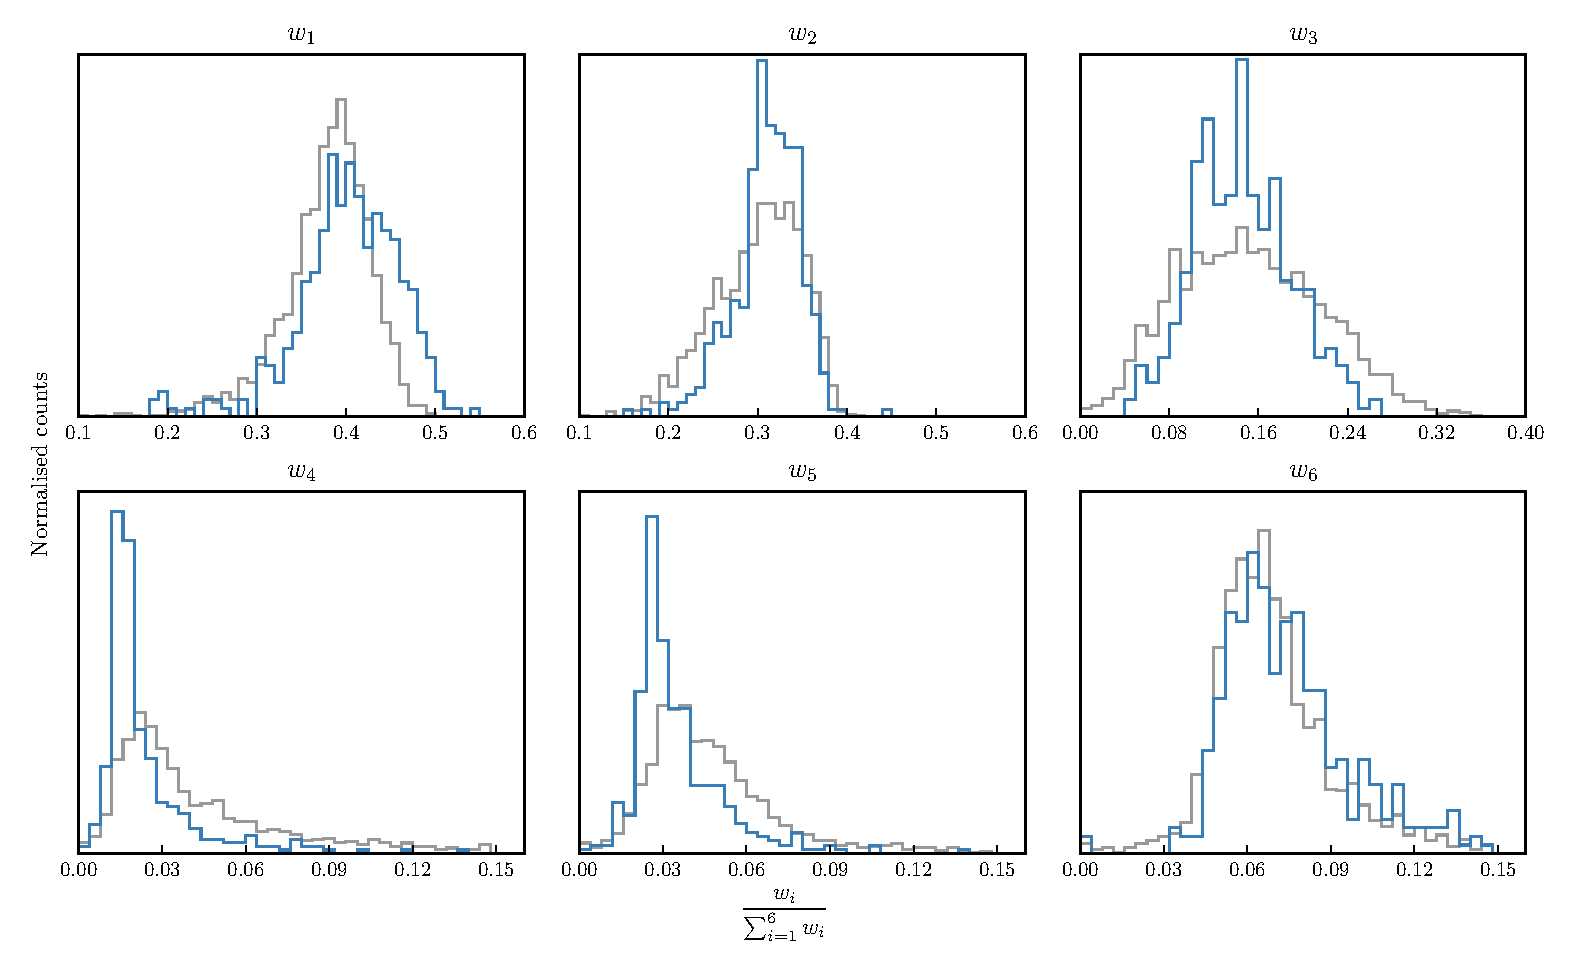
\includegraphics[width=\textwidth]{figures/chapter04/mfica_component_weights.pdf} 
    \caption[{The relative weight in each of the six positive ICA components for the high-luminosity and low luminosity samples.}]{The relative weight in each of the six positive ICA components for the high-luminosity (blue) and low luminosity samples (grey). In the high-luminosity sample \ion{Fe}{II} emission is stronger (component $w_1$). The core [\ion{O}{III}] emission (components $w_4$, $w_5$) is weaker but the strength of the blueshifted wing ($w_6$) is the same.}     
    \label{fig:mfica_component_weights}
\end{figure}

\begin{figure}
    \captionsetup[subfigure]{labelformat=empty}
    \centering
    \subfloat[\label{fig:mfica_oiii_weight_a}]{}
    \subfloat[\label{fig:mfica_oiii_weight_b}]{}
    \subfloat[]{{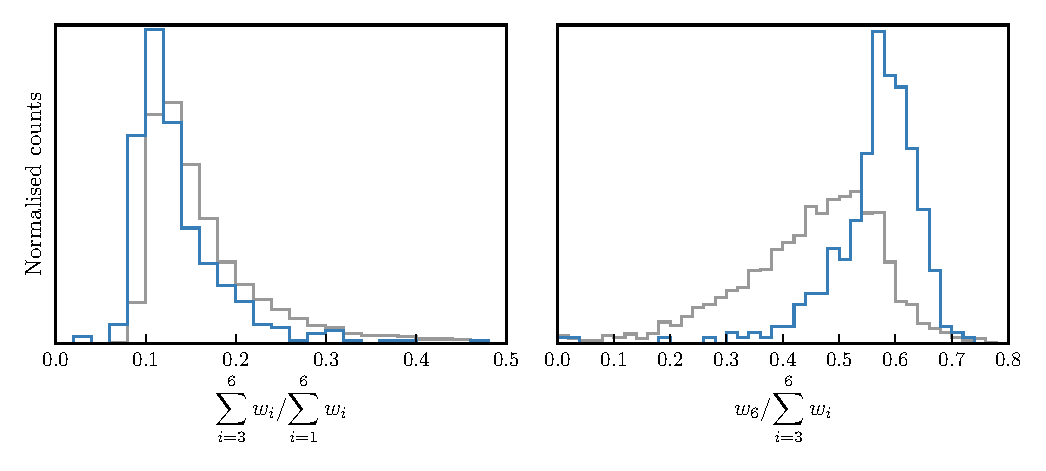
\includegraphics[width=\textwidth]{figures/chapter04/mfica_oiii_weight.pdf} }}
    \caption[{The relative weight in the three ICA components corresponding to [\ion{O}{III}] emission and the relative weight of the component most closely related to blueshifted [\ion{O}{III}] emission relative to all three [\ion{O}{III}] components.}]{The relative weight in the three ICA components corresponding to [\ion{O}{III}] emission ({\em left}) and the relative weight of the component most closely related to blueshifted [\ion{O}{III}] emission relative to all three [\ion{O}{III}] components ({\em right}). [\ion{O}{III}] emission is weaker in the high-luminosity sample, but the relative contribution from the blueshifted component to the total [\ion{O}{III}] emission is higher.}     
    \label{fig:mfica_oiii_weight}
\end{figure}

\begin{figure}
    \centering
    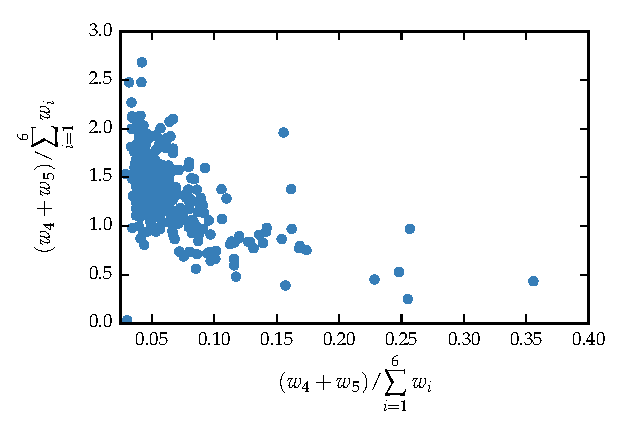
\includegraphics[width=\columnwidth]{figures/chapter04/oiii_core_strength_blueshift.pdf} 
    \caption[{Weight in the [\ion{O}{III}] wing relative to the weight in the [\ion{O}{III}] core emission versus the strength of the core [\ion{O}{III}] emission.}]{Weight in the [\ion{O}{III}] wing relative to the weight in the [\ion{O}{III}] core emission versus the strength of the core [\ion{O}{III}] emission. The blue-asymmetry of the [\ion{O}{III}] emission increases as the strength of the core component decreases.}     
    \label{fig:oiii_core_strength_blueshift}
\end{figure}

In Figure~\ref{fig:mfica_component_weights} we show the relative weights of each of the six positive ICA components. 
Also shown are the same measurements for a sample of low-redshift, low-luminosity AGN. 
We want to examine whether or not there are systematic differences between these two samples. 
\todo{Paul: Paragraph belongs with material above}

We see that [\ion{O}{III}] core emission is weaker in the more luminous sample, but the strength of the wing component is similar. 
\citet{shen14} showed that the strength of the core [\ion{O}{III}] component decreases with quasar luminosity and optical \ion{Fe}{II} strength faster than the wing component, leading to overall broader and more blueshifted profiles as luminosity and \ion{Fe}{II} strength (or \ion{C}{IV} blueshift) increases. 
\citet{shen14} suggested that a stable NLR is being removed by the outflowing material. 
Similarly, \citet{zhang11} found that the more the peak of the [\ion{O}{III}] line is blueshifted, the more the core component decreases dramatically, while the blue wing changes much less. 
Therefore, there is an anti-correlation between the strength of the core component and the relative strength of the wing component (Figure~\ref{fig:oiii_core_strength_blueshift}). 

To show this phenomenon more clearly, we plot the relative [\ion{O}{III}] strength and the [\ion{O}{III}] wing/core ratio in the high/low luminosity samples (Figure~\ref{fig:oiii_core_strength_blueshift}). 
We see that [\ion{O}{III}] is weaker in the high luminosity sample, but that the wing component is much stronger relative to the core component. 
\todo{Similar to behaviour of \ion{C}{IV}? Would suggests that the mechanism producing the two correlations is the same}. 

\subsubsection{EV1 correlations}

\begin{figure}
    \centering
    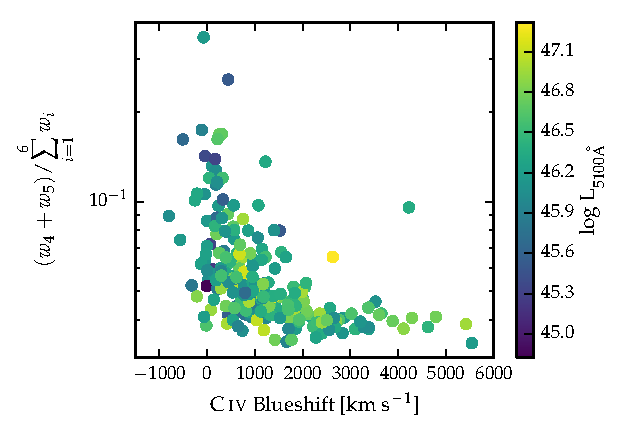
\includegraphics[width=\textwidth]{figures/chapter04/civ_blueshift_oiii_strength.pdf} 
    \caption[{The ICA component weight $w_4$, which is a proxy for the strength of core [\ion{O}{III}], as a function of the \ion{C}{IV} blueshift.}]{The ICA component weight $w_4$, which is a proxy for the strength of core [\ion{O}{III}], as a function of the \ion{C}{IV} blueshift. The \ion{C}{IV} blueshift is measured relative to the near-infrared ICA redshift.}     
    \label{fig:civ_blueshift_oiii_strength}
\end{figure}

\begin{figure}
    \centering
    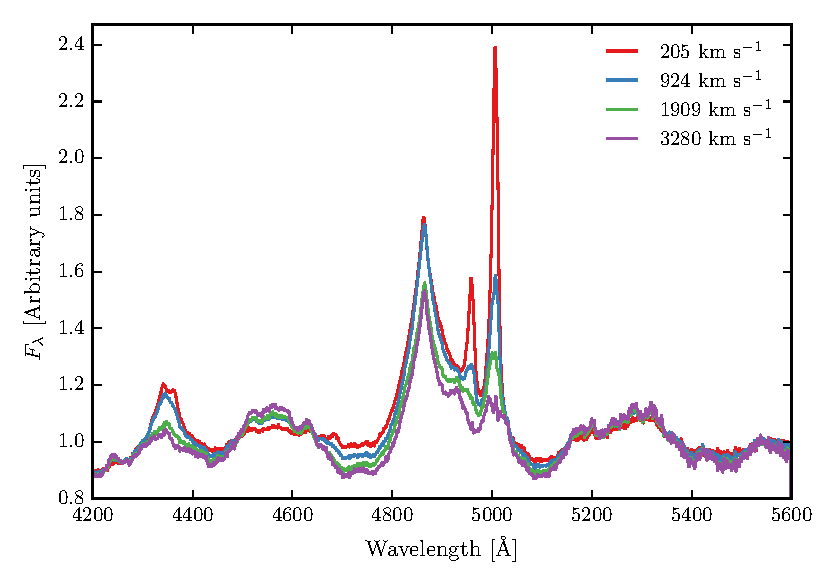
\includegraphics[width=\columnwidth]{figures/chapter04/mfica_composites.pdf} 
    \caption[{Median ICA-reconstructed spectra as a function of the \ion{C}{IV} blueshift.}]{Median ICA-reconstructed spectra as a function of the \ion{C}{IV} blueshift.}     
    \label{fig:mfica_composites}
\end{figure}

In Figure~\ref{fig:civ_blueshift_oiii_strength} we show how the [\ion{O}{III}] strength varies as a function of the \ion{C}{IV} blueshift. 
There is a very well defined relation: when \ion{C}{IV} is strongly blueshifted [\ion{O}{III}] is very weak. 
This is very similar to what we found when we used Gaussian functions to model the emission. 
The correlation between \ion{C}{IV} blueshift and [\ion{O}{III}] EQW is shown in a different way in Figure~\ref{fig:mfica_composites}. 
Here we divide our sample into four bins according to the \ion{C}{IV} blueshift. 
From the quasars in each \ion{C}{IV} blueshift bin we then find then generate an ICA spectrum using the median weights from each quasar. 
The differences in the spectra as a function of the \ion{C}{IV} blueshift are dramatic. 
[\ion{O}{III}] becomes progressively weaker and more blueshifted.
The anti-correlation with \ion{Fe}{III} and the blue-ward \ion{Fe}{II} also clear, but there is no change in the redward \ion{Fe}{II}. 

\subsubsection{Updating EV1}

The ICA can be thought of as update on EV$1$.
EV$1$ is a quest for HR diagram for quasars - clearly very important.  
The spectral diversity is encapsulated in the EV$1$ components. 
Most of the variance in EV$1$ is the anti-correlation between the strengths of [\ion{O}{III}] and \ion{Fe}{II}. 
So at one end we have objects with strong \ion{Fe}{II} and weak [\ion{O}{III}], and at the other end objects with weak \ion{Fe}{II} and strong [\ion{O}{III}]. 
Other properties, including the \ion{C}{IV} blueshift and the \hb FWHM, also change systematically. 
Our work shows that the ICA component weights change systematically along the EV$1$ sequence. 

\todo{Just present this as an idea for future work right at the end rather than having this sandwiched in the middle.} 

Accurate systemic redshift estimates are essential in a number of applications, and researchers have devoted a large amount of telescope time to obtaining near-infrared spectra to access [\ion{O}{III}] for this purpose. 
HI, CO and absorption-line measures of the host-galaxy rest frame suggest that [\ion{O}{III}] usually gives consistent results within $200$\,\kms\, (de Robertis 1985; Whittle 1985; Wilson \& Heckman 1985; Condon et al. 1985; Stripe 1990; Alloin et al. 1992; Evans et al. 2001).  
However, our work shows that at high luminosities this can result in large errors (profile can be dominated by blueshifted component, \ion{Fe}{II} emission can be improperly subtracted, or [\ion{O}{III}] might not be detected at all. 
[\ion{O}{III}] is weaker and broader so it is more difficult to detect and measure [\ion{O}{III}] accurately for these luminous quasars (to for instance obtain reliable redshift estimates based on [\ion{O}{III}])

\subsection{Future work}

Pros:

It is less sensitive to the spectral S/N, and the component weights do not need to be constrained. 
It is therefore much simpler to apply than fitting multiple Gaussians. 

Cons:

The components were calculated using a set of lower-redshift, lower-luminosity AGN, and quasar spectra are known to vary systematically as a function of luminosity. 
For example, the [\ion{O}{III}] line is typically broader in more luminous quasars. 
Because there are so few objects with very broad [\ion{O}{III}] in the low-redshift sample, the ICA reconstruction fails to reproduce the broadest [\ion{O}{III}] profiles in our sample. 

Cross-talk between components. 






The size of the narrow line region is roughly expected to scale as $L^{0.5}$ \citep[e.g.][]{netzer04}. 
However, for high luminosity quasars with strong [\ion{O}{III}] this gives NLR sizes which are unreasonably large \citep[$\sim100$ kilo-parsec;][]{netzer04}. 

\todoinline{See extra text from Brotherton paper. I could be confused here, but I think the Netzer argument goes that the nlr size increase with luminosity because there are more ionising photons. but then you run out of nlr to ionise. the luminosity of the quasar keeps increasing but the luminosity of the nlr flattens out. so the eqw starts to decrease. but we see a huge scatter in eqw at high luminosities. we can relate this to the \ion{C}{IV} blueshift, which I don't think Netzer will have been able to.}



We see a correlation between the [\ion{O}{III}] velocity width and asymmetry. 
As the line gets broader it gets more blue-asymmetric. 
One interpretation of this is that the strength of the narrow core is decreasing, leading to a broader and more blueshifted profile \citep[e.g.][]{shen14}. 


[\ion{O}{III}] is broader, which is consistent with these quasars having more massive BHs. 
[\ion{O}{III}] also shows stronger blue asymmetries, suggesting that outflows are stronger/more prevalent at these higher luminosities/redshifts. 
The luminous blueshifted broad wing and the extremely broad profile reveals high-velocity outflowing ionized gas. 
Our results therefore suggest that kilo-parsec-scale outflows in ionized gas are common in this sample of high-luminosity, high-redshift quasars.



\section{Radio}

Radio properties would be interesting. 
Have another look, and at least say we tried and there aren't enough objects.


% Looking at the [\ion{O}{III}] velocity width as a function of luminosity tells us about the physical drivers of the outflows observed in [\ion{O}{III}]. 
% The correlation with luminosity suggests that the highest velocity outflows are associated with the most luminous AGN. 
% This has been reported for low-redshift AGN, for both ionized and molecular outflows (e.g. Westmoquette et al. 2012; Veilleux et al. 2013; Arribas et al. 2014; Cicone et al. 2014; Hill \& Zakamska 2014).

% This suggests that the outflows are driven by radiative forces. 
% On the other hand, \citet{mullaney13} find that once the correlation between the [\ion{O}{III}] luminosity and the radio luminosity has been taken into account, the [\ion{O}{III}] velocity width is more strongly related to the radio luminosity of the AGN. 

\section{Summary}

At fixed luminosity, I find that as the blueshift of the \ion{C}{IV} emission increases, the [\ion{O}{III}] emission becomes weaker and more blueshifted, and disappears entirely in quasars with the most extreme \ion{C}{IV} blueshifts.  